\chapter{Introduction}
\label{chap:Intro}
There are many tools on the internet that help with visualizing data. Some of them also help to create networks to show relations between numerous items. Famous examples are "ConceptDraw Pro", "Lucidchart" \cite{JeffParker} or "draw.io". However when using these the user spends a lot of time on creating a nice looking diagram, centering important components etc., to get a pleasant looking result in the end.

The idea for this project is to offer an online editor with CRUD-functionality for a network, consisting of components of software projects, as well as a first implementation of an algorithm that will, in most cases, create a nice looking layout on its own.

\section{Purpose}
The purpose is to try out and test a combination of technologies. This software, or variations of it, might later be incorporated into a bigger project or adapted to fit another use case. The experiences and impressions during development can be of help when thinking about what technology stack to use, which is why a big part of this paper is dedicated to documenting this process.

\section{The Endresult}
To give the reader a better understanding of the context lets quickly look at the application at the end of this project.
\begin{figure}[H]
\centering
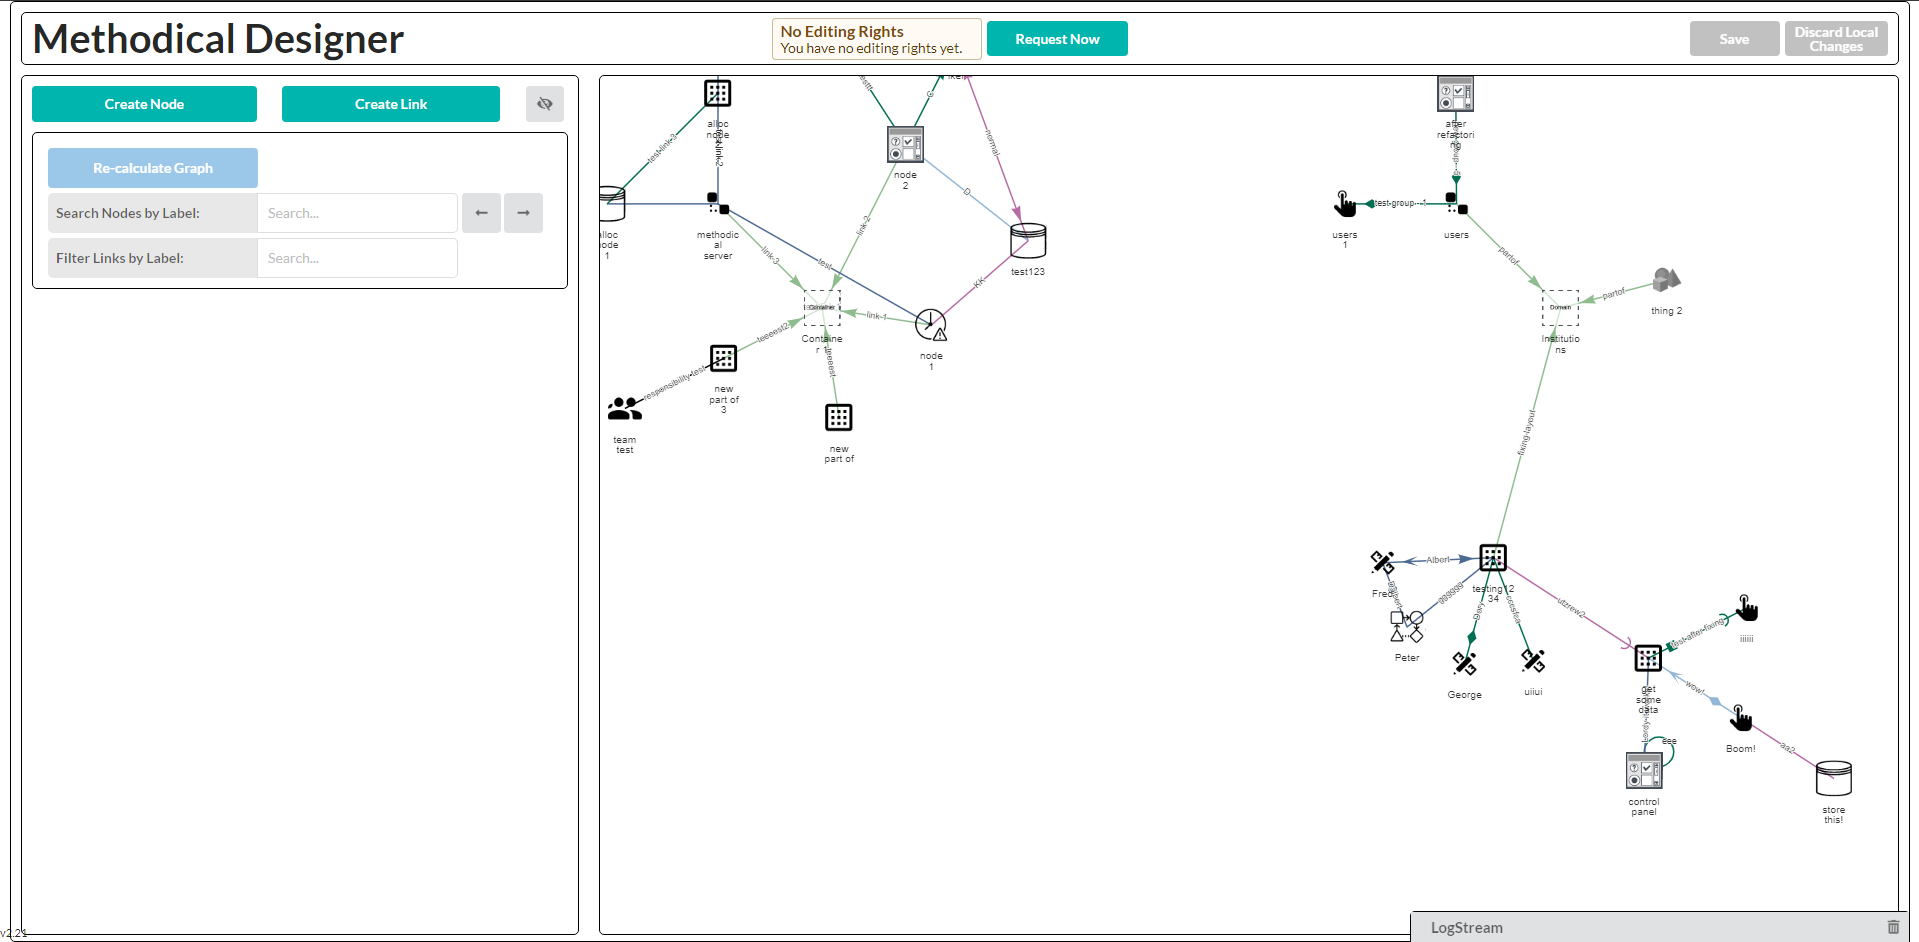
\includegraphics[scale=.35]{Bilder/AppOverview.png}
\captionof{figure}{The Application}
\label{pic:AppOverview}
\end{figure}

The top bar contains buttons that communicate with the server. Initially it is not possible to make changes to the data. Another person might currently be editing the graph and two people editing the graph at the same time might lead to not compatible changes. When clicking the \emph{Request Now} button the server will check if editing rights for the project are already taken. If not the server will send the newest data from the database to make sure the latest changes are shown to the user, otherwise the user will be informed.

Should he make local changes the two buttons on the top right become clickable and allow to permanently save changes to the database or discard all changes and reset the local set to the one in the database.

The left pane contains buttons for the user to interact with the application. Clicking the buttons to create nodes and links will display the respective form.
Furthermore there are fields to search nodes and filter the links that are displayed in the canvas on the right and a button that will re-calculate the layout of the graph when the data has changed.

When selecting a node or link the pane on the left will show a form containing all saved data. Should the user have editing rights he can also make changes and save them. There are different node and link types, where each can but must not have a different syntactical meaning.

\section{Definitions}
The word \emph{graph} refers to a network of nodes that are connected through links. Nodes must not be connected to links, but each link must be connected to a node (it can be the same one twice) on each end. This means that there can be various not connected networks of nodes and links in one graph.

A \emph{collapsable} is a node that can hide (collapse) its children and show (expand) them if they should have a \emph{Part-Of} link to such node. In this nodes of two types have this functionality: Containers and Domains. The button to do so appears in the form on the left if the user selects a collapsable node.

\chapter{Backend to Frontend}

This chapter will introduce the individual components, tools and frameworks this application is built with. For some of them it will give some more insights on how they work internally, others are so big that a detailed description would go beyond the scope of this paper. The order will be the same as they appeared in the development process.

\section{The GRAND-stack}
GRAND stands in this case for \textbf{G}raphQL, \textbf{R}eact, \textbf{A}pollo and \textbf{N}eo4j \textbf{D}atabase. \cite{GrandStackGettingStarted} React is a frontend framework, Apollo is used for statemanagement on the client side and communicating to the database on the server side. GraphQL will be used for the communication between them. Neo4j is a graph database and the server will communicate with it through a JavaScript driver provided by the Neo4j community.

\section{Query Language - GraphQL}
GraphQL is a data query language as well as specification. Its development was started by Facebook in 2012 and it was open sourced in 2015. \cite{GraphQLFoundation}

After their application suffered from poor performance on mobile devices, they took a new implementation using natively implemented models and views. This required a new API for their news feed as it was previously delivered as pure HTML. \cite{EngineeringFB}

After evaluating different common options like RESTful-APIs and Facebook Query Language (FQL) they often saw the same problems:  The ratio of data actually used compared to the one fetched was very small, the number of requests \cite{GraphQLIntro} and the amount of code on both server and client side to prepare the data was big. \cite{EngineeringFB}

For example, for loading the start page of a single user, there would have been a lot of different requests necessary:
\begin{itemize}
\item \emph{https://facebook.com/user/id} - Get all user specific data
\item \emph{https://facebook.com/user/id/events} - Get all possibly relevant events
\item \emph{https://facebook.com/user/id/friends-suggestions} - Get all friend suggestions
\item ...
\end{itemize} \cite{GraphQLIntro}

GraphQL aims to resolve all these issues: Reduce the amount of unnecessary data transferred, reduce the number of requests and increase the developer productivity by making it easier to use fetched data. \cite{EngineeringFB}

It allows developers to get a lot of different data from a single endpoint. This means that instead the above shown 3+ endpoints, when using GraphQL all requests would go to \emph{graph.facebook.com}, with a query similar to:\\
\newpage
\lstset{language=GraphQL}
\begin{lstlisting}[caption={A GraphQL Query to Fetch User Data},label={ex211}]
query {
	user(id: 1) {
		name
		events {
			count
		}
		friends_suggestions {
			name
			mutual_friends {
				count
			}
		}
	}
}
\end{lstlisting}
\citep[with adaptions]{GraphQLIntro}	
Where the answer would be a JSON-string:
\begin{lstlisting}[caption={Example Response Data},label={ex212}]
{ 
	"data": {
		"user": {
			"name": "Brandon Minnick",
			"events": {
				"count": 4
			},
			"friends_suggestions": {
				"name": "Seth Juarez",
				"mutual_friends": {
					"count": 18 
				}
			}
		}
	}
}
\end{lstlisting}
\citep[with adaptions]{GraphQLIntro}	

The query can be as extensive as the developer needs it, it will return only the data requested and the answer string can be directly accessed like a JSON-object. By that GraphQL fulfills all its design goals.
\\ \\
The previously shown query then needs to be resolved by a server thats able to interpret GraphQL and resolve the query. All non primitive data types have to be defined following the GraphQL specification. An example for a user schema might be:
\newpage
\begin{lstlisting}[caption={Type Definition in GraphQL}]
type User {
	id: ID! 
	name: String! 
	events: [Event] 
	friends: [Friend] 
	friends_suggestions: [Friend_Suggestion] 
}
\end{lstlisting}

\noindent
where "Event", "Friend" and "Friend\_Suggestion" themselves are other types described in a similar manner.

By putting a "!" behind a property it is marked as required, meaning it can never be null or empty. The square brackets define that the property is a list of the type they surround.

To be able to run queries in the first place, it is necessary to first define a root type for all queries:

\begin{lstlisting}[caption={Root Type Definition}]
schema {
	query: Query
}
\end{lstlisting}

In this root type all possible queries must be described:

\begin{lstlisting}[caption={Defining Queries}]
type Query { 
	user(id: ID!): User 
}
\end{lstlisting}

This describes a query that can be executed as shown in \autoref{ex211} by providing an ID to the query and the correct query name, together with a collection set telling the server which fields to fetch. In the parentheses any query arguments are listed, in this example id must be provided. After the colon the return type is named. 

The server will then make requests to the DB, fetch the requested data and return it to the user once all fields were filled with values.

%For further information about the extensive type system please see the official GraphQL specification. \cite{GraphQLSpec}

\section{Database - Neo4j}
\subsubsection{General}
Neo4j is a so called graph database. The idea of graph databases is, compared to traditional relational databases, a young concept and differs in a few concepts. At the moment Neo4j is the 22nd most popular database overall \cite{DbEnginesGeneral} and the most popular graph database. \cite{DbEnginesGraph}

\begin{itemize}
\item Unlike most relational databases, who store data through tables and joins, Neo4j stores data in the form of actual nodes and relationships between such \cite{Neo4jDevGuides}. In other DBMS relations between items generally are achieved through join-/lookup-tables which have to be generated. \cite{RelVsGraph}

\item When running a query on a graph DB the server will index only once to find the initial node \citep[minute 32]{NeoInternals}. All related nodes can be directly accessed through their relationship with the current one. \cite{WhatGraphDB} These are stored as memory pointers which makes following them extremely efficient.

\item Neo4j uses Cypher as query language. The Cypher syntax visually represent the shape of the data a user wants to retrieve instead of describing how to get data, as well as offer the power and functionality other languages offer. \cite{Neo4jCypher} 
\end{itemize}

\subsubsection{Cypher}
For matching all nodes connected to node A through a "Neighbor" relationship, simply state
\lstset{language=Cypher}
\begin{lstlisting}[label={ex231},caption={Matching Nodes Way 1}]
MATCH (n:Node {label: "A"})-[:Neighbor]-(n2:Node) RETURN n, n2
\end{lstlisting}
Parentheses represent a node, square brackets a relationship. The naming works after the following pattern: <name>:<type>. In this example n is the name for the first node and n2 the name of the list of connected nodes. Specifying a name for the relationship is not necessary as no data will be retrieved from it. Specific properties a node or relationship should have can be specified within curly braces. Another query with the same result set would be
\begin{lstlisting}[label={ex232},caption={Matching Nodes Way 2}]
MATCH (n:Node)-[:Neighbor]-(n2:Node) WHERE n.label = "A" RETURN n, n2
\end{lstlisting}
which might look a bit cleaner. It is also possible to return only specific values of n and n2 and give them names by stating
\emph{ ...RETURN n.label AS Label1, n2.label AS Label2 }

The following information about Neo4j internals is all from \cite{NeoInternals} and \cite{Neo4jInternalsPP}. Sadly, these sources are all old and probably outdated, yet there does not seem to be more updated information available.

\subsubsection{The Graph on Disk}
Internally, there are 3 types of records saved on the disk: node-, relationship- and property-records. All of these have fixed sizes to allow for quicker allocation during the start up process. Every record has an "inUse" field, as well as a unique ID with which Neo4j is able to exactly locate a searched record on the disk. \citep[minute 08]{NeoInternals}

Properties on nodes are saved through a linked list like object. The exact implementation however does not alter the idea behind it. A property knows about its type and has a next pointer. Each node saves the pointer to its first property whose next pointer will lead to the next property etc.. Should a next pointer be empty the algorithm knows that it has reached all properties of a node.

In addition to the first property, each node knows about its first relationship. If it is the \emph{first} one, it is simply being determined by the order of creation. A relationship has pointers to its start- and end-node, to its type and four more to other relationships, which are best explained in an example traversal in pseudo code:
\newpage
\lstset{language=JavaScript}
\begin{lstlisting}[caption={Algorithm to Save Read the Graph from Disk}]
if node n has relationship pointer r: 
	if n is start node of r: 
		if r has StartNext pointer sn: 
			set r = sn 
			repeat from line 2 
		endif 
		else  
			visited all relationships $ \rightarrow $ terminate
		endelse 
	endif 
	else 
		if r has EndNext pointer en: 
			set r = en 
			repeat from line 2 
		endif 
		else
			visited all relationships $ \rightarrow $ terminate
		endelse 
	endelse 
endif
\end{lstlisting}

This shows that every relationship has two next pointers. Which one will be used for further traversal, depends on if the source node is start- or end-node in the current relationship.

In addition to this, the same pointers exist into the other direction, meaning that there are also two pointers called StartPrevious and EndPrevious. The question for selecting which one will be chosen for further iteration stays the same.

\subsubsection{The Graph in Memory}
Upon start up these records are being loaded into the "FS Cache" (File System Cache). Neo4j will then partition these into equally sized regions and create a hit counter for each of them, to encounter high traffic regions that will be loaded into the "Node/Relationship Object Cache" which is more similar to an actual graph. \\
Here each node holds a list of relationships that are grouped by the relationship type to allow for quick traversals, and relationships only hold their properties as well as start- and end-node and their type. Any references to other records are being done by its ID. 

\subsubsection{Traversing}
For finding a node to start traversing the graph, Neo4j uses traditional indexing. \citep[minute 32]{NeoInternals} Once the start node is found, 2 concepts take over:
\begin{enumerate}
\item \textbf{RelationshipExpanders} which will for a node return all relevant relationships to continue traversing from that node
\item \textbf{Evaluators} which return if traversing should continue on this branch ($ \rightarrow $ expand) or not and if this node should be included in the result set or not.
\end{enumerate}
When accessing a node the first thing the system will try to do is fetch it from the cache. If it isn't be there, the next place that will be checked is the FS Cache. Should the region that contains the node be available there, the access is quick but blocking, meaning that the entire region is getting locked. In the case that the region is out of the FS cache the operation is blocking and slower. \\
The locking is necessary to make sure that no other transaction will evict that area from the memory while the current one reads from it.

\subsubsection{Adding Cypher}
As Cypher describes the shape of the searched data, a searched query will be converted into a representative pattern graph. This is an internal representation of a valid result set that matches the searched structure. Found patterns will be compared to it to decide whether they should be included in the result set or not.

When a query is run, the first thing that happens is that matching start-nodes are searched in the database (through indexing). When a node is found, traversing the database starts as described above. For Expanders and Evaluators to know what to return, they simply compare the pattern graph described through Cypher with the graph that was found so far and see if there is more data that matches. 

\section{Server - ApolloServer}
%maybe some general information about Apollo?
Apollo Server is a spec-compliant GraphQL server. It can be embedded into Node.js middleware like Express or Fastify \cite{ApolloServerIntro} and will listen for connections on a defined port. \\
When it receives one it will read the query and call the respective route, or resolvers as they are called. \\
In addition to that the server will deliver, together with some more, a \emph{context} object to each route that contains a driver which connects to a database, which is Neo4j in our case. Using this object together with a specified Cypher query allows the manipulation of the DB. 

\subsubsection{Example Resolver}
A resolver to create a node might look like the following:

\begin{lstlisting}[caption={A Basic Resolver},label={ex241}]
async CreateNode( _, args, ctx ) { 
	const session = ctx.driver.session(); 
	const query = ` 
			CREATE (n:Node:${ args.nodeType } {id:$id, label:$label, nodeType: $nodeType}) 
			SET n += $props 
			RETURN n`; 
	const results = await session.run(query, args);
	return results.records.map(record => record.get('n').properties)[0]; 
}
\end{lstlisting}

The following describes each step:
\begin{itemize}
\item Line 1 contains the function definition. "args" is an object that contains all data sent with the query from the frontend. "ctx" is the context object that contains the neo4j driver to communicate with the DB. The first argument "\_", which is a placeholder here as it is not needed, is the so called "parent" which is equal to the previous resolver in the resolver chain. (More about this in the next section)
\item Line 2 acquires a session to communicate with the database. \cite{Neo4jDriver} This object allows sending Cypher queries to the database that get executed right away.
\item Lines 3 to 6 define a Cypher query which is similar to the ones shown in \autoref{ex231} and \autoref{ex232}. 
\item In line 4 makes use of the args object and embeds the nodeType directly into the query string by using template strings. This is necessary because at this position of a cypher query it is not possible to make use of query variables as in the rest of the query. This line also shows that by using \$<variableName> query variables that were passed along can be accessed.
\item Line 5 demonstrates the usage of an object that can be passed as query variable. This object can't only contain simple datatypes, but its really useful to set various values at once.
\item Finally, line 7 sends the specified query string together with the args object (that must contain all referenced variables) to the database. Using the ES6 await keyword makes sure that code execution doesn't continue until the results are returned.
\item The last line iterates over the record set and retrieves any properties by the in the query specified name. Using only the first element of the array is specific to this case, as CreateNode is defined to return a single node, not an array of such.
\end{itemize}

\subsubsection{Resolver Chain}
To explain the resolver chain lets take a look at the following example GraphQL query: \citep[with adaptions]{ApolloResChain}
\lstset{language=GraphQL}
\begin{lstlisting}[label={ex242},caption={GraphQL query to fetch all books with their title and author name of all libraries}]
query GetBooksByLibrary {
	libraries { 
		branch 
		books { 
			title 
			author { 
				name 
			} 
		} 
	} 
}
\end{lstlisting}

\newpage
which will be executed on this schema \citep[with adaptions]{ApolloResChain}
\begin{lstlisting}[caption={Schema Definition},label={ex243}]
# A library has a branch and books 
type Library { 
	branch: String! 
	books: [Book!] 
} 

# A book has a title and author 
type Book { 
	title: String! 
	author: Author! 
	branch: String! 
} 

# An author has a name 
type Author { 
	name: String!
} 

type Query { 
	libraries: [Library] 
}
\end{lstlisting}

\noindent
To resolve the query there are 4 resolvers necessary:
\begin{itemize}
\item A root resolver which defines the entry point for the query
\item One resolver each for "Library", "Book" and "Author"
\end{itemize}

\noindent
Assuming that there are static arrays called "libraries", "books" and "authors" available that are filled with data, the resolvers might look like the following: 
\citep[with adaptions]{ApolloResChain}
\newpage
\lstset{language=JavaScript}
\begin{lstlisting}[caption={Resolver Definition},label={ex244}]
const resolvers = { 
	Query: { 
		libraries() { 
			return libraries; 
		} 
	}, 
	Library: { 
		branch( parent ) { 
			return parent.branch; 
		}, 
		books( parent ) { 
			return books.filter( book => book.branch === parent.branch ); 
		} 
	}, 
	Book: { 
		title( parent ) { 
			return parent.title; 
		}, 
		author( parent ) { 
			return authors.find( author => author.name === parent.author.name ); 
		} 
	}, 
	Author: { 
		name( parent ) { 
			return parent.name; 
		} 
	}
};
\end{lstlisting}

First, the Query resolver is hit and it will search for a defined key that is similar to the name mentioned in the highest level of the query object in \autoref{ex241}, in this case "libraries". The GraphQL schema under \autoref{ex243} defined that this query will return an array of Library objects.

Knowing this, the server will now go through each object of this array and look for resolvers of the in the query specified fields. This object is passed as \emph{parent} into the next resolver in the resolver chain.

For each library the server has to get the branch and an array of books. As branch is a primitive type it does not need to be further resolved. Books however, returns an array of non-primitive types. To find out which books need to be returned it is enough to use the value of \emph{parent.branch} and compare it to the branch of each book in the books array and return those who match.

Books is again an array of a non primitive type and has to be further resolved by iterating through the array and accessing the requested values title and author. Title is just a string, whereas author will get resolved further, etc.
\newpage
\subsubsection{Cypher in GraphQL}
Using GraphQL directives it is possible to "annotate" our schema and specify precisely certain actions or checks the server should perform when accessing a field. \\
The following schema shows the definition and usage of a directive: \cite{GraphQlDir}

\lstset{language=GraphQL}
\begin{lstlisting}[caption={Example Directive Declaration}]
directive @deprecated( 
	reason: String = "No longer supported" 
) on FIELD_DEFINITION | ENUM_VALUE 

type ExampleType { 
	newField: String 
	oldField: String @deprecated(reason: "Use `newField`.")
}
\end{lstlisting}

Directives can be distinguished by the @-symbol and are placed after a field definition to annotate one. When querying \emph{oldField} on \emph{ExampleType} the server might only respond with "Use 'newField'" and not send any data. The exact behavior depends on how directive behavior is defined in the server.

The use cases range from formatting strings, enforcing access permissions to value checking when the client sends data and many more. 
%For information about how directives can be implemented please refer to \cite{GraphQlDir}

Using the GRAND-stack allows the usage of a pre-defined directive called "@cypher" and through that use cypher statements directly in the schema definition file. A great and short example is getting all connected nodes for a specific node:

\begin{lstlisting}[caption={Cypher in GraphQL}]
type Node { 
	... 
	connectedTo: [Node] @cypher(statement: "MATCH (this)--(:Link)--(n:Node) return n") 
	...
}
\end{lstlisting}

The node that is currently being iterated over in the resolver chain is passed as \emph{this} to Neo4j. Then it'll look for other nodes that are connected through any relationship of type \emph{Link} and return these. In addition to this, there's an npm package that can generate default resolvers for queries and mutations meaning there is no need to write a resolver for \emph{Node} manually. This makes writing query resolvers a rare occasion when using the GRAND-stack. \\

Please note that this feature of using the cypher queries in the schema is only available when \emph{APOC} is installed on this Neo4j instance.

\newpage
\section{Frontend - React}
React is a JavaScript-Framework to create component-based user interfaces. Each component has to define a \emph{render} method which describes what appears on the screen. In this method the programmer writes basic HTML or can embed other react components. \\
The standard \emph{index.html} is pretty short when using react. The only code a programmer writes there is normally in the header area to include CDNs or other resources. The body contains only one element: \\
\emph{<div> id="root"></div>} 

\subsubsection{Components}
In \emph{index.js} this root div will be referenced by the react-internal render method and recursively build the basic html out of the defined react components:
\lstset{language=HTML}
\begin{lstlisting}[caption={index.html for Hello World},label={ex250}]
<!DOCTYPE html>
<html>
<head>
	<title>Intro-App</title>
</head>
<body>
	<div id="root"></div>
</body>
</html>
\end{lstlisting}

\lstset{language=JavaScript}
\begin{lstlisting}[caption={Hello World in React},label={ex251}]
// index.js:
ReactDOM.render(
	<App/>,
	document.getElementById( 'root' ),
);
// App.js:
import React from 'react';

class App extends React.Component {
	render() {
		return (
			<div>
				Hello World
			</div>
		);
	}
}

export default App;
\end{lstlisting}

A class component is defined by extending from \emph{React.Component}. Each class component must at least have a \emph{render()} method. React will use the return values of these methods to build the DOM.

When starting the react app, opening it in the browser and selecting inspect the following is the output in the "Elements" tab (ignoring a script for live updates in the head):

\lstset{language=HTML}
\begin{lstlisting}[caption={Resulting HTML after building}]
<html> 
<head>
	<title>Intro-App</title>
</head>
<body>
	<div id="root">
		<div>
			Hello World!
		</div>
	</div>
</body>
</html>
\end{lstlisting}

React starts traversing at whatever component is put into the \emph{ReactDOM.render} method and repeats the process for each component until primitive html elements that can be rendered directly are reached.

Every React class component can receive values from its parent element, by passing them like normal html property (e.g. line 3 below). In the child they can be accessed through a variable called \emph{props} and with JSX it is possible to embed the value of variables directly in the component (e.g. line 14 below):

\lstset{language=JavaScript}
\begin{lstlisting}[caption={Using Props},label={ex252}]
// index.js:
ReactDOM.render(
	<App text={ 'Hello World' } />,
	document.getElementById( 'root' ),
);

// App.js:
import React from 'react';

class App extends React.Component {
	render() {
		return (
			<div>
				{ this.props.text }
			</div>
		);
	}
}
export default App;
\end{lstlisting}
Both \autoref{ex251} and \autoref{ex252} will produce the exact same output.

\subsubsection{State}
React class components have a state which can be used to manage user actions on a component, as well as general application data. \emph{state} is a simple JavaScript object but should be treated as immutable and only be updated through the \emph{setState()} method. Modifying the state directly can lead to bugs and/or unexpected behavior of the application.

To demonstrate this, lets take a look at a \emph{Counter} component in the application (code does not contain imports and exports):

\begin{lstlisting}[caption={Counter Component}]
// index.js
ReactDOM.render(
	<App text={ 'Hello World' }/>,
	document.getElementById( 'root' ),
);

// App.js
class App extends React.Component {
	render() {
		return (
			<div>
				{ this.props.text }
				<Counter/>
			</div>
		);
	}
}

// Counter.js
class Counter extends React.Component {
	constructor( props ) {
		super( props );
		this.state = { val: 0 };
		this.increase = this.increase.bind( this );
		this.decrease = this.decrease.bind( this );
	}

	increase( e ) {
		e.stopPropagation();
		let { val } = this.state;
		val++;
		this.setState( { val } );
	}

	decrease( e ) {
		e.stopPropagation();
		let { val } = this.state;
		val--;
		this.setState( { val } );
	}

	render() {
		return (
			<div>
				<p>Current score: { this.state.val }</p>
				<button onClick={ this.increase }>+</button>
				<button onClick={ this.decrease }>-</button>
			</div>
		);
	}
}
\end{lstlisting}

When defining a custom constructor for a class component it is necessary to call \emph{super( props )} first. Defining an initial state can be done by setting \emph{this.state = \{ val: 0 \}}. This is the only place where state should modified directly. In comparison to that before updating state in lines 32 and 39 the app first creates a copy of the value it will modify by using Object Destructuring and then call \emph{this.setState( \{ val \} )} to update it. By doing so it does not modify the state object directly.

Lines 24 and 25 bind the this keyword on the increase and decrease functions. Not doing so and accessing \emph{this.setState()} in any of the methods would crash the application as \emph{this} would be the global window object which doesn't have a \emph{setState} method defined.

The render method defines the output of the component. It'll render a paragraph telling the current score by accessing the state together with two buttons and their respective click handlers.

\subsubsection{Updating Components}
React is known for its good performance \cite{LinaSpukas} even in large applications. To understand better how it achieves this, this section will look a bit at the internal process of rendering and updating the components. \\

On the initial render React will create a component tree from which it'll then build the DOM that the browser converts into displayable objects and paints them on the screen. To show how react determines which part of the DOM it has to update, lets quickly walk through the previous example:

When clicking the increase or decrease button in the previous example the components state gets updated which will automatically trigger a re-render. In such a small component it wouldn't really matter if React simply rendered the whole component. In a component containing hundreds of lines and probably many other sub-components the decision to render all of it just because would take a long time and be fatal for performance. Especially if really all it'd have to do is re-render line 45.

\subsubsection{Finding The Differences}
To know what exactly to update, React performs something called \emph{Reconciliation}. This process is very complicated, so this explanation leaves out the details and explain it in a few steps: 
\begin{itemize}
\item The \emph{setState} function will mark the component and all its children as dirty. \cite{GethylGeorgeKurian}
\item It'll recursively walk through all components marked as dirty, building them in the virtual DOM \cite{GethylGeorgeKurian}
\item For each built element it compares it to the value in the actual DOM. Depending on what changed (type, HTML attributes, keys, etc.) it will either destroy and replace or modify them.  \cite{ReactDocs} 
\end{itemize}
By doing so, instead of re-rendering the whole \emph{Counter} component it only re-renders
\begin{lstlisting}[caption={Updated line}]
<p>Current score: { this.state.val } </p>
\end{lstlisting}

\subsubsection{Stateless Functional Components}
It is also possible to create stateless functional components. In their pure form they do not contain state and normally only show either static data or data they get passed through props. The \emph{App} component in the above examples does exactly that. Knowing this, it could be re-written:
\begin{lstlisting}[caption={App as Functional Component}]
// App.js
import React from 'react';
import Counter from './Counter';

function App( props ) {
	return (
		<div>
			{ props.text }
			<Counter/>
		</div>
	);
}
export default App;
\end{lstlisting}
Which is a lot shorter and has another big advantage: It protects from laziness. \cite{CoryHouse} As this component doesn't support local state it is not too tempting to quickly hack something new into it. Rather the programmer gets encouraged to think about the structure and create a proper component for a new feature together with its own state object that only that component needs.

And of course visually the result is equal to the one in \autoref{ex251} and \autoref{ex252}.

\newpage
\section{Client - ApolloClient}
ApolloClient is a state management library for JavaScript that manages data with GraphQL. It offers an all in one solution for fetching, caching and modifying application data and together with automatic UI updates upon events from the server. \cite{ApolloClientIntro}

\subsubsection{Hooks}
ApolloClient 3 offers this by providing custom \textbf{hooks}. Hooks are a new addition to React since React 16.8 and were introduced to improve stateless functional components \cite{ReactHooksIntro} and can only be used in such. \cite{ReactHooksOverview} There were a few reasons that led to the introduction of hooks like the appearance of complex class components that couldn't be split into smaller ones, not re-usable stateful logic and classes being not ideal for future optimization. \cite{ReactHooksIntro} Hooks allow for example the usage of state in functional components.

\subsubsection{Apollo Hooks}
In addition to some built-in Hooks provided by React it is also possible to create them. Apollo implemented many of its own hooks, the focus here will be on \emph{useQuery}, \emph{useLazyQuery} and \emph{useMutation}.
The first argument to all of these is a GraphQL string. A query for the first two, a mutation for the last one.

The second argument is the options object. By adding properties to this the execution behavior can be influenced. Probably the most important argument is \emph{variables}. This is an object containing key-pair values that equal to the ones used in a GraphQL query as shown in \autoref{ex211}. In addition to that there are \emph{onError} and \emph{onCompleted}. These are two callback functions that allow for executing actions upon completion or handling of possible errors. Imagine \emph{GET\_DATA} being a valid GraphQL query string:
\begin{lstlisting}[caption={The useQuery Hook from Apollo}]
function Test() {
	useQuery( GET_DATA, {
		variables: { id: 1 },
		onCompleted: data => console.log( data );
		onError: error => console.log( error.message );
	} );
	...
}
\end{lstlisting}

%For the rest of the arguments please refer to API reference form Apollo.

To be able to use returned data and inform the user about the current status, all of these three hooks return a few other objects, the most important being \emph{data}, \emph{loading} and \emph{error}. These are boolean values and allow for conditional rendering inside a component, depending on their values:
\newpage
\begin{lstlisting}[caption={Demonstration of the useQuery Hook}]
function Test() {
	const { data, loading, error } = useQuery( GET_DATA, {
		...	
	} );
	
	if ( loading ) return 'Fetching data.';
	if ( error ) return 'Error when fetching data.';
	return 'Success!';
}
\end{lstlisting}

In comparison to \emph{useQuery} the other two also return a function object that can be called upon specific a action to execute the query or mutation (see example below).

The \emph{useMutation} hook is the only one of the three allowing for an \emph{update} argument in the options object. In this it is possible to access the local cache and have access to the results returned from the mutation. This can be useful if local data in the cache needs to be updated depending on the result of a server operation:
\begin{lstlisting}[caption={Creating a Mutation and defining a manual update function},label={ex:usingMutation}]
function Mutate() {
	const [ runMutation, { data, loading, error } ] = useMutation( DO_THING, {
		update: ( cache, { data } ) => {
			// update cache with return data from mutation
		}	
	} );
}
\end{lstlisting}
This approach works well and is more or less the only way of handling return results from external mutations. 

\subsubsection{Local Resolvers}
The same could be done for local state changes, but as these functions can become long it might clutter the component with a lot of code that is not actually for it. To get rid of this problem the client allows the definition of local resolvers:
\begin{lstlisting}[caption={Local Resolvers},label={ex253}]
const client = new ApolloClient({
	...,
	resolvers: {
		Mutation: {
			setData: ( _, variables, { cache } ) => {
				// manage local state update			
			},
			...		
		},	
	},
	...,
});
\end{lstlisting}

Just like when calling a query or mutation on the server it is necessary to define a GraphQL query to call it:
\lstset{language=GraphQL}
\begin{lstlisting}[caption={Query Definition for a Mutation in the Client}]
const SET_DATA = gql`
	mutation SetData($data: [String]!) {
		setData(data: $data) @client	
	}
`;
\end{lstlisting}
The name in line 3 has to match with the one defined in the resolver in \autoref{ex253} in line 5. But whats even more important is the \emph{@client} directive at the end of line 3. This tells Apollo to not contact the server, but rather resolve the mutation locally. The above defined mutation can be called like this:
\lstset{language=JavaScript}
\begin{lstlisting}[caption={Using the Client Side Mutation}]
const Test() {
	const [ runSetData ] = useMutation( SET_DATA );
	
	const handleClick = e => {
		e.stopPropagation();
		runSetData(	{ variables: { data: 'test' } } );
	}
	
	return (
		<button onClick={ handleClick }>Click me</button>
	);
}
\end{lstlisting}

\subsubsection{The Apollo Cache}
A feature of Apollo is its smart cache. Once a query to the server has been executed, the results are saved in the cache and should the exact same query be executed again, the cache will first check if it has results for this query saved locally. If so, it'll return them from there, reducing network traffic and improving performance of the whole application. 

Of course in some cases it might be necessary to always have the newest data from the cache. The exact behavior can be specified through the \emph{options} object passed to a query or mutation.

\chapter{Deployment}

While developing in a local environment it is also important to test the application in a production environment as early as possible. Many frameworks make optimizations to improve performance. This might lead to errors that can't be seen in a local setup. Often they also change error behavior. While during development an error might only lead to a warning message, in production the same error might cause the application to crash.

Another reason to go for early deployment is to allow other people to see, use and test the application. Someone who sees the app for the first time or at least doesn't know how things were thought to work will make completely different use of it than a programmer. New issues with the workflow can be discovered and problems that a developer would never have thought of may be discovered. Further the layout will be tested on different screens, browsers and devices, unveiling unknown layout troubles. Issues discovered early are much easier to fix than those who are integrated deeply into the codebase. \\

This chapter will introduce the tools that were used to deploy the application to a publicly available cloud platform that allows it to be used and tested by anyone, anywhere.

\section{Docker}
Docker is a platform that provides the ability to a developer to create any environment in which he wants to execute code in.
Before comparing it to a virtual machine lets take a look at the basic terminology:

A \emph{Docker File} is a text file containing instructions that tell the Docker Engine how to build a \emph{Docker Image}. \cite{NickDocker}

This \emph{Docker Image} is a file containing necessary data to execute a given program. The in the docker file specified libraries are saved, folders from the local machine are copied, environment variables are set etc.. 

Running the image will start a \emph{Docker Container}. It will execute specified commands and by that for example download node modules. This container is an instance executed by the \emph{Docker Engine} which runs on top of the Host OS of an actual machine.

\newpage
While it is similar to a virtual machine, there are certain differences between them: \\
\textbf{Operating System} Every VM comes with its own operating system, making it heavy in terms of memory and processing power they require. Docker containers in turn all share the hosts operating system and only require the docker engine to be installed on the machine: \cite{GeekDocker}
\begin{figure}[H]
\centering
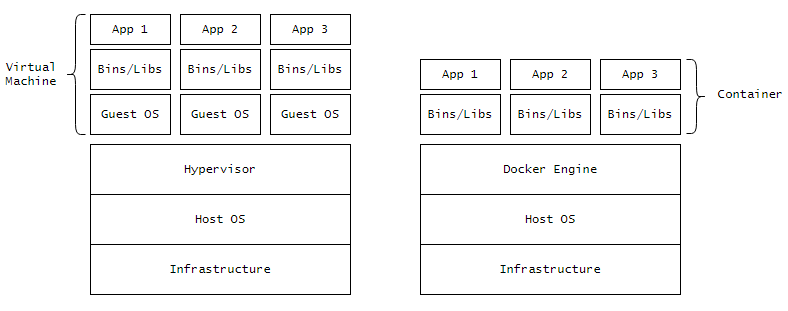
\includegraphics[scale=.8]{Bilder/DockerVsVM.png}
\captionof{figure}{Virtual Machine vs. Docker}
\label{ex312}
\end{figure}
\noindent
\textbf{Security} Following the previous point, every VM has its own operating system and is strongly isolated in the host kernel. Docker containers all run on a single kernel. Furthermore docker resources are shared. If an attacker gets access to one container he'll be able to exploit  all containers in a cluster. \cite{GeekDocker}) \\
\textbf{Portability} Containers can easily be ported to any machine that has the docker engine installed. There is no further configuration necessary, they'll run the same on any machine. VMs are more difficult to port just due to their sheer size. In addition, the process of setting up a virtual machine differs from operating system to operating system. 

\section{AWS}
AWS is a cloud platform from Amazon that offers over many different services in various geographic regions around the world. This project made use of 3 of them to make the application publicly available. This section will give a short introduction and overview over each of them.

\subsection{AWS-EC2}
EC2 is a service that allows the creation of virtual machines with over 300 different variations of computational capacities like the number of CPUs, Memory, Storage and Network Performance. \cite{AwsEc2} 
Available configurations that can run on an instance are called Amazon Machine Images (AMIs) and include various Linux based distributions like Ubuntu, Debian or fedora as well as Windows. In addition to empty operating systems Amazon and different communities also provides images with certain pre-installed software making sure that instances can be set up quickly.
Basically, an EC2 instance is a virtual machine that runs on an Amazon server. \cite{Ec2VirtualMachine}

%In this app we will make use of EC2 to run a Neo4j instance. To make configuration easier, the Neo4j community provides images that can be started directly with only a few clicks from the AWS EC2 management console. By selecting AMIs and searching for "neo4j-community" in public images we can see all the available images with different versions of Neo4j. We will select one of the images that contains \emph{apoc} in their name to be able to use Cypher in our GraphQL schema. After clicking Launch we can select an instance https://neo4j.com/developer/neo4j-cloud-aws-ec2-ami/
\newpage
\subsection{AWS-ECS}
ECS is a service to run automatically managed docker containers on AWS servers. Many big companies make use of this service because of its scalability, reliability and security. \cite{AwsEc2}
These are the most important terms when talking about AWS ECS: \\

A \textbf{Task Definition} is the blueprint of a task, specifying which Docker image(s) to use, ports to expose, can set environment variables and memory needed etc. \cite{CodeCampEcs}

A \textbf{Task} is an instance that is created following the specifications in the task definition. A task can run various Docker containers at once. A task is where an application actually gets executed.

A \textbf{Service Description} is the blueprint for a service. It contains for example the minimum and maximum number of tasks running at once, as well as thresholds to when changes to the number of running tasks should happen and other specifications.

A \textbf{Service} is an instance that is created following the specifications in the Service Description. One service can run various tasks at once and use a load balancer to distribute network traffic equally over all running tasks.

A \textbf{Cluster} is a logical grouping of services. \\

These components can be visually put together as shown in \autoref{ex311}. \citep[with adaptions]{AwsEcs} \\

\begin{figure}[h]
\centering
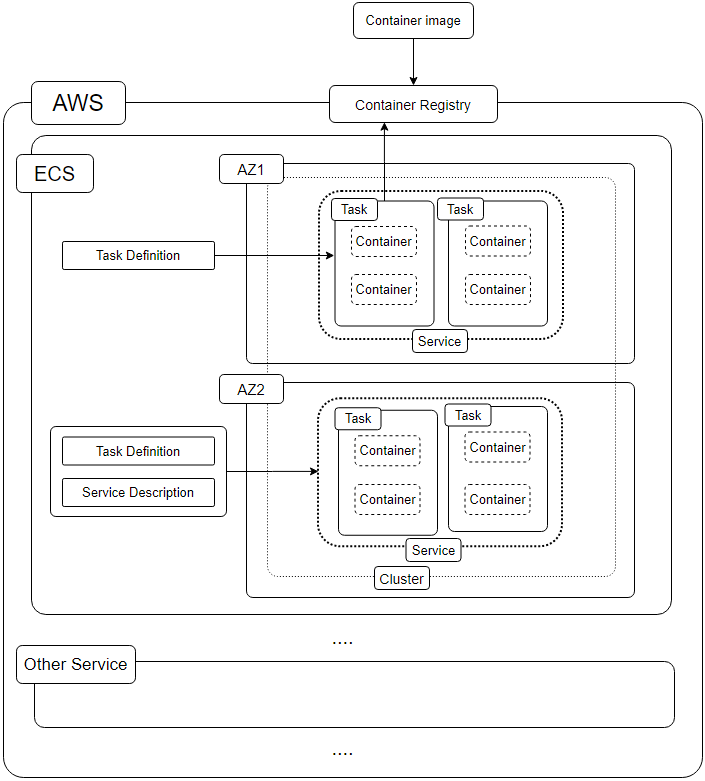
\includegraphics[scale=.8]{Bilder/EcsStructure.png}
\captionof{figure}{Structure of AWS ECS}
\label{ex311}
\end{figure}

A task is created from a task definition and placed in a service. It is possible to allow AWS to automatically manage all Docker and VM resources and then run the docker image directly. The dashed box is a cluster. This cluster contains 2 services, reach running 2 tasks running 2 containers. 

The services of a cluster can be run in different \emph{Availability Zones} (AZ), meaning that they run on servers from AWS located in different parts of one geological region to improve response time.

\subsection{AWS-Amplify}
Amplify is a service that aims to make the development as well as the deployment of applications as easy as possible. It comes with many advanced features that help setting up an app quickly. Some examples are: Authentication, API creation, Analytics, Push Notifications and many more \cite{AwsAmplify}. It creates a certificate for any deployed application, allowing for HTTPS connections. Further it is able to scan a connected GitHub repository and provide a template configuration based on the framework used.

Another really nice feature is the easy deployment flow: For each application it is possible to connect various branches. Each branch will have its unique URL and once a developer pushes to a connected branch, Amplify will build the newest status of the application. This is a great feature for testing new features in a production environment without having to deploy to a master environment directly.

\chapter{Development}
This discussion is not a "how to" guide because in the course of this work some mistakes were made. This section describes key architectural decisions and reports equally on those which turned out well and those which turned out badly.

Workarounds found for certain problems should not be considered best practice but rather as hint to a solution if one of these problems should appear in similar projects.

The examples in this chapter are taken from the actual application, unless stated otherwise.

\section{Why the GRANDstack}
To find out which tech stack to use, the first step was to analyze what the application should be able to do:
\begin{itemize}
\item The app will be interactive, not purely informational
\item The user will create, modify and delete data
\item Local changes made to data can be saved permanently
\item Data must be displayed as graph
\item At some point one might want to be able to implement real time updates that show changes made by another user
\end{itemize}
This will give a list of requirements our tech stack should fulfill:
\begin{itemize}
\item Updating the DOM should be done efficiently as the layout needs to update with almost every user action
\item A local state management will be needed to keep track of local changes
\item A database will be necessary to permanently save changes
\item An intuitive way for saving graph data
\item Communication with the server should be lightweight and easy to implement
\end{itemize}

Having looked at the individual parts of the GRANDstack, it becomes clear that it contains many things that could be useful: Neo4j is a graph database, actually saves a graph on disk and is extremely performant. GraphQL only transmits the data needed when communicating with the server. Together with Apollo, which offers a lot of help when implementing subscriptions, live updates should not be too hard to realize. Subscriptions are a way of keeping a communication channel between server and client, making sure the server can inform all listening clients about an incoming event.

Having a state management framework and a backend server that are designed to work together also promises for a trouble free development. The Apollo hooks make it very intuitive to update the UI according to state changes.

Furthermore this stack contains many relatively new an immature technologies and as mentioned in \autoref{chap:Intro} this project also serves to explore these.

\section{The GraphQL Schema}
Development of applications that leverage GraphQL usually start by creating a schema to define the shape of data. The good thing about this is that it can be adapted if during the process it comes up that actually changes are necessary.

This part will take a brief look at the GraphQL schema this app uses and mention a few things that didn't work out as expected when creating it.
\lstset{language=GraphQL}
\begin{lstlisting}[caption={GraphQL Enums},label={enums}]
enum NodeType{
  API
  Command
  Query
  Event
  Persistence
  AbstractUserInterface
  Object
  Computation
  Container
  Domain
  Invariant
  ArchitecturalDecisionRecord
  Definition
}

enum LinkType{
  PartOf
  Trigger
  Read
  Mutate
  Generic
}

enum ArrowType{
  Default
  none
  SharpArrow
  Curve
  Diamond
  Arrow
  Box
  Triangle
  Bar
  InvTriangle
}
\end{lstlisting}
Any node will have a type from the \emph{NodeType} enum above. The type decides how the node will be displayed in the application. What values are part of this enum depends on what the app should display. The same counts for links and the \emph{LinkType} enum. Furthermore every link can have arrows of different shape on each end. As this app uses a canvas library to take care of the drawings on the screen the values that are part of this enum depend on what the library offers.

\begin{lstlisting}[caption={Usage of Interfaces in GraphQL}]
interface IDisplayable{
  id: ID!
  label: String
  story: URI
}

type Node implements INode & IDisplayable{
  id: ID!
  label: String!
  nodeType: NodeType!
  story: URI
  Links: [Link] @cypher(statement: "MATCH (this)--(l:Link) RETURN l")
  synchronous: Boolean
  unreliable: Boolean
  connectedTo: [Node] @cypher(statement: "MATCH (this)--(:Link)--(n:Node) return n")
}
  
type Link implements ILink & IDisplayable{
  id: ID!
  label: String!
  linkType: LinkType!
  x: Node! @cypher(statement: "MATCH (this)-[:X_NODE]->(n:Node) RETURN n")
  y: Node! @cypher(statement: "MATCH (this)-[:Y_NODE]->(n:Node) RETURN n")
  x_end: LinkEnd @cypher(statement: "MATCH (this)-[:X_END]->(le:LinkEnd) RETURN le")
  y_end: LinkEnd @cypher(statement: "MATCH (this)-[:Y_END]->(le:LinkEnd) RETURN le")
  sequence: SequenceProperty @cypher(statement: "MATCH (this)-[:IS]->(s:Sequence) RETURN s")
  story: URI
  optional: Boolean
}

\end{lstlisting}
Coming from an Object Oriented background using interfaces seemed intuitive. Having an ID, label and story object to be apparent on all entities that can be shown on screen makes sense. What was not known when creating the schema is that visjs requires each link to be connected to an x and y node, in other words: a link can't "float". This means that there are two more required fields in the ILink interface, making the IDisplayable interface conflict with its purpose of defining properties that are required to be displayed.

The \emph{@cypher} directive shown earlier can be used to easily retrieve the links attached to the node. This is an array which can be empty as nodes do not necessarily need be connected in any way. The same idea holds for the array of connected nodes. The two booleans \emph{synchronous} and \emph{unreliable} were subject to a lot of discussion as they could also be placed on links rather than nodes to annotate them.

\emph{optional} on link is a value that would have been used for template functionality that is not implemented yet in the application.

\begin{lstlisting}[caption={Input Type Definitions}]
type SequenceProperty{
  group: String
  seq: Int
}

input NodeInput{
  label: String
  story: URI
  nodeType: NodeType
  synchronous: Boolean
  unreliable: Boolean
}

input NodeCreateInput{
  synchronous: Boolean
  unreliable: Boolean
  story: URI
}

type LinkEnd{
  note: String
  arrow: ArrowType
}
\end{lstlisting}
If more than one link connects the same pair of nodes a sequence property can be used to assign a group id to each link and an order within that group. Because of that each sequence on a link contains a string identifying the sequence group it belongs to as well as a sequence number to display the order in which steps will be executed. Each link end can contain a note about how the component on the respective end perceives the incoming connection.

The input types are used to be able to pass an object into GraphQL queries or mutations instead of just primitive datatypes. This idea sounds promising as one can just pass all input objects from a form to the query. In the end it turned out that this led to a lot of object modifying just to get the right structure from the input types which is why the usage of these input types was not worth the effort. In this case it would've been better to put all input values directly into a \emph{variables} object that gets sent to the server.

\newpage
\begin{lstlisting}[caption={Mutation Type Definition},label={mutations}]
type Mutation{
  SeedDB: seedReturn
  CreateNode(id: ID!, label: String!, nodeType: NodeType!, props: NodeCreateInput): NodeOperationReturn
  CreateLink(id: ID!, label: String!, x_id: ID!, y_id: ID!, linkType: LinkType!, props: LinkCreateInput): LinkOperationReturn
  CreateSequence(link_id: ID!, props: SequencePropertyInput): SequenceOperationReturn
  CreateLinkEnd(link_id: ID!, props: LinkEndInput): LinkEndOperationReturn

  MergeSequence(link_id: ID!, props: SequencePropertyInput): SequenceOperationReturn
  MergeLinkEnd(link_id: ID!, props: LinkEndInput): LinkEndOperationReturn

  UpdateNode(id: ID!, props: NodeInput): NodeOperationReturn
  UpdateLink(id: ID!, props: LinkInput): LinkOperationReturn
  UpdateSequence(link_id: ID!, props: SequencePropertyInput): SequenceOperationReturn
  UpdateLinkEnd(link_id: ID!, props: LinkEndInput): LinkEndOperationReturn

  DeleteNode(id: ID!): deleteReturn
  DeleteLink(id: ID!): deleteReturn
  DeleteSequence(link_id: ID!): deleteReturn
  DeleteLinkEnd(link_id: ID!, xy: String!): deleteReturn

  RequestEditRights: EditRightOperationReturn
  FreeEditRights: EditRightOperationReturn
}
\end{lstlisting}

This is the definition of the root mutation type. It clarifies even more the previously made point of having a lot of trouble formatting the inputs for a mutation: When dispatching a \emph{CreateNode} mutation two of the form inputs (label and nodeType) have to be passed directly, while all others need to be put into an object called props that contains the fields defined in the respective input type. This makes the code for form handling a lot harder to re-use, especially as the input types vary for updating and creating.

\newpage
Lets talk about the return types defined for each operation:
\begin{lstlisting}[caption={Return Types}]
interface IReturnInfo{
  success: Boolean!
  message: String
}
type NodeOperationReturn implements IReturnInfo {
  success: Boolean!
  message: String
  node: Node
}
type LinkOperationReturn implements IReturnInfo{
  success: Boolean!
  message: String
  link: Link
}
\end{lstlisting}
Similar to how a project using a REST-API would implement it, this was the idea of the process:
\begin{itemize}
\item Frontend dispatches a call to the server
\item Server starts resolving
\item Resolving is successful
	\begin{itemize}
		\item Server sets \emph{success} to true and adds the created object to the payload
	\end{itemize}
\item Resolving fails
	\begin{itemize}
		\item Server sets \emph{success} to false and adds an error message
	\end{itemize}

\item Frontend checks \emph{success} and depending on its value will either display data about the modified object(s) or the error message defined by the server
\end{itemize}

Maybe it was due to missing experience, but it didn't seem intuitive at all to define custom responses from the ApolloServer to the client. Just by accident the manner to return custom error messages appeared, but it was already late in development process and there was not enough time left to build it into all places where it would've been necessary. More about this in \autoref{chap:LB}.

\begin{lstlisting}[caption={Root Type Definitions}]
type Query{
  Nodes: [Node]
  Links: [Link]
  IsProjectBeingEdited: EditRightQueryReturn
}

schema {
  mutation: Mutation
  query: Query
}
\end{lstlisting}

The end of the schema contains the definition for the query type and the root schema.

\section{Getting started with Neo4j}
To get started with Neo4j its a good idea to first create a small basic data set that shouldn't be too complicated to be able to easily experiment with it. So lets try to create a representation of the following graph in the database:

\begin{figure}[H]
\centering
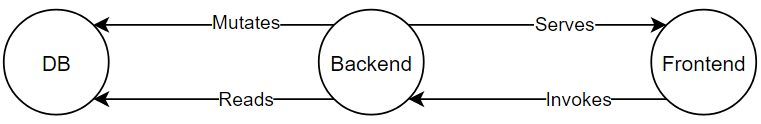
\includegraphics[scale=.8]{Bilder/BasicGraph.png}
\captionof{figure}{A small network of software components used for testing}
\label{ex421}
\end{figure}

The goal is to display this graph in the application. It is really helpful to first draw it on paper and then think of the individual components needed. As there will be one graph in the database and one in the application it is important to carefully separate them when talking about a node: While a node in the app is always a node in the database, this is not necessarily the case the other way around as a node in the database could also represent data about a connection in the application.

This code will create the three nodes for DB, Backend and Frontend:
\lstset{language=Cypher}
\begin{lstlisting}[caption={Cypher Statements to Create the Nodes}]
CREATE (:Node:AbstractUserInterface {id: randomUUID(), label: "Frontend", story: "Interaction point for the user", nodeType: "AbstractUserInterface"})
CREATE (:Node:API {id: randomUUID(), label: "Backend", story: "Endpoint for requests, fetches from and mutates data on the DB", nodeType: "API"})
CREATE (:Node:Persistence {id: randomUUID(), label: "DB", story: "Saves data for the methodical designer", nodeType: "Persistence"})
\end{lstlisting}

Everything between the parentheses of a create statement defines a new node in Neo4j. By using colons one defines labels for a node. These can be used to filter for a certain type of node and can improve performance when traversing. 

All of them are of type node and each of them has its own specific label, marking them as different node types. Curly braces are used to define properties on each of them: A unique ID for each node by using Neo4j's \emph{randomUUID()} function, a label which will be displayed in the application and a story which shortly describes its functionality for each node. Furthermore each node receives a nodeType. This might seem a bit counter intuitive as this was already defined in the Neo4j labels for the node.
Later on when retrieving the nodes from the database its only possible to get all of those, which would be a list like \emph{[Node, API]}. For displaying it however only one of them is necessary. To be able to easily extract it, it has its own property on each node.

\newpage
This is how the created graph looks like in the Neo4j Browser:
\begin{figure}[H]
\centering
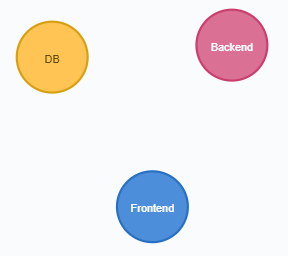
\includegraphics[scale=1]{Bilder/BasicGraphNeo1.png}
\captionof{figure}{The nodes in Neo4j Browser}
\label{ex422}
\end{figure}

Before directly creating the respective connections between the nodes to complete the data for the image lets first think about what properties such a link might contain later:
\begin{itemize}
\item Data about the x-end of the connection (arrow-type, color, an annotation about how the x-node component sees the connection)
\item The same for the y-end
\item Information about if the link is part of a sequence of steps and if so a short description of the step
\item A label, id, story and linkType
\item The IDs of the nodes it connects
\end{itemize}

One option would be to save all this information on the relationship between the nodes. But if the user now updates only the label of a node and saves this change, the frontend will send all fields and the DB will have to write all other properties as well without actually modifying them.

To somewhat minimize the amount of data sent it might be a good idea to split the information among various nodes:
\begin{itemize}
\item One link-node that containing the label, id, story and linkType
\item Two link-end-nodes containing visual information about the arrow as well as a "note" field to clarify how one node might perceive the connection
\item One sequence-node to specify whether or not the node is part of a sequence
\end{itemize}

The link-node would have direct connections to the components it connects. The sequence- and link-end-nodes would be connected to their link-node and can be accessed by finding the link and from there looking for respective connections.

Having this in mind lets go on to create the link-nodes and attach them to their components. For now lets not create any sequence- or link-end-nodes to keep things simple:

\begin{lstlisting}[caption={Creating and Connecting the First Link}]
MATCH (api:API) WHERE api.label = "Backend"
MATCH (db:Persistence) WHERE db.label = "DB"
CREATE (l:Link)
SET l.label = "Mutates", l.linkType = "Mutate", l.story = "See JIRA for details: https://.."
CREATE (api)<-[:IS_X]-(l)-[:IS_Y]->(db)
\end{lstlisting}

This code will find a node with an \emph{API} label and one with a \emph{Persistence} label. It can be taken for granted that this will find the correct nodes in this example because only one of each type exists. Normally their node IDs would be necessary to identify them. Putting a string in front of the first colon in the match case will declare a variable name for the found node which can be used later to reference it. Then the code will create a link from api to DB, giving it a \emph{Link} label and assigning the link the variable name \emph{l}. This variable is used to set the link's properties label, linkType and story. This time the story serves as reference to an external document describing the relationship in more detail. Then using another create statement Neo4j will create a connection between the link-node (a Neo4j node representing a link in the application) and the node-node (a Neo4j node representing a node in the application). After executing the Neo4j Browser will show the following image:
\begin{figure}[H]
\centering
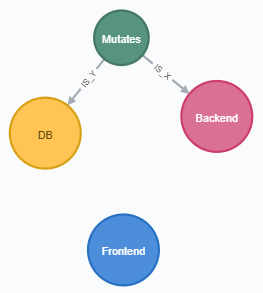
\includegraphics[scale=1]{Bilder/BasicGraphNeo2.png}
\captionof{figure}{After creating the first link-node}
\label{ex423}
\end{figure}

\newpage
After adding the rest of the connections using the same approach the whole representation on the data layer looks like:
\begin{figure}[H]
\centering
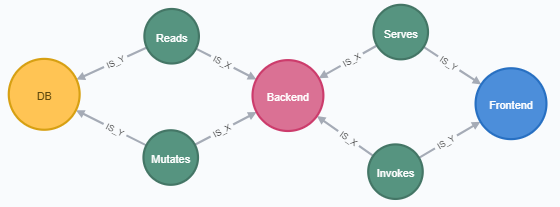
\includegraphics[scale=1]{Bilder/BasicGraphNeo3.png}
\captionof{figure}{Whole graph in the DB}
\label{ex424}
\end{figure}

To make this more clear lets compare it to the graph to be displayed in the app:
\begin{figure}[H]
\centering
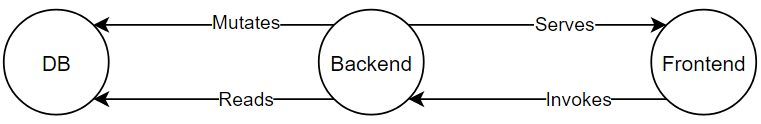
\includegraphics[scale=.8]{Bilder/BasicGraph.png}
\captionof{figure}{A small network of software components used for testing}
\label{ex:GraphSideBySide}
\end{figure}

The yellow, pink and blue circles represent the nodes that are also shown as nodes on the frontend. The connections and all data they contain have turned into the green circles. It is important to note that directions of the arrows in \autoref{ex424} do not represent the direction of the link in the image. They are only necessary because Neo4j doesn't allow for undirected links in create statements. To make it uniform all relationships were made to be outgoing from the link nodes.

To shorten the example the information about the arrows in \autoref{ex:GraphSideBySide} does not exist in \autoref{ex424}. 

\section{Communicating with the DB through ApolloServer and GraphQL-Playground}
The next step is to communicate with the database through the server. After setting up ApolloServer (more on setup in \autoref{chap:Doc}) a first step would be to create a resolver to seed the database with some default data similar to the one shown previously in \autoref{ex423}. This was really helpful as especially in the beginning making mistakes which can leave the dataset in a bad shape is common and fixing it manually would take a lot of time. Line 2 in \autoref{mutations} contains the GraphQL definition. 
\newpage
The resolver looks like the following:
\lstset{language=JavaScript}
\begin{lstlisting}[caption={Seed Resolver}]
const seedQuery = require( './seed' );
async SeedDB( _, __, ctx ) {
	try {
		const session = ctx.driver.session();
		const deleteQuery = 'MATCH (n) DETACH DELETE n';
		await session.run( deleteQuery );
		await session.run( seedQuery );
		await session.close();
		return {
			success: true,
		};
	}
	catch( e ) {
		return {
			success: false,
		};	
	}
},
\end{lstlisting}

The \emph{seedQuery} is a long cypher query defined in an external file. After deleting all nodes and connections in the database using the \emph{deleteQuery} it gets executed to create new data to use.

To run this resolver and seed our database the following GraphQL query can be used in the GraphQL Playground:
\lstset{language=GraphQL}
\begin{lstlisting}[caption={Seeding the DB through GraphQL Playground}, label={exSeed}]
mutation seedDB {
  SeedDB {
    success
  }
}
\end{lstlisting}
The name in line 1 is completely optional. What matters is line 2 as this string will be used to identify the correct resolver. Tthe curly braces are used to define a result set. After hitting the play button the expected result gets returned:
\begin{lstlisting}[caption={Seeding Result}, label={exResSeed}]
{
  "data": {
    "SeedDB": {
      "success": true
    }
  }
}
\end{lstlisting}

The next step is retrieving data. As mentioned previously, to save some time when writing queries, one can use use the neo4j-graphql-js npm package which combines resolvers and a GraphQL schema to an executable schema. This package can generate many queries and mutations based on the schema provided but still allows the usage of custom resolvers.
By doing so, nodes can be fetched without any further coding:

\begin{lstlisting}[caption={Fetching Nodes}, label={exFetch}]
query nodes {
  Nodes {
    id
    nodeType
    label
  }
}
\end{lstlisting}

With the result being similar to:
\begin{lstlisting}[caption={Result Set}, label={exResFetch}]
{
  "data": {
    "Nodes": [
      {
        "id": "738e414d-bc1f-4e90-ad76-ec44d34f1a71",
        "nodeType": "AbstractUserInterface",
        "label": "UI"
      },
      {
        "id": "6c4b4dba-5726-47bc-8fb5-10affcf03ef7",
        "nodeType": "API",
        "label": "Server"
      },
      {
        "id": "2554b296-ffed-4028-ad80-1181dfe97ecd",
        "nodeType": "Persistence",
        "label": "NeoDB"
      },
      {
        "id": "ded515d5-8016-4324-a756-201b9e1f2db0",
        "nodeType": "Event",
        "label": "Create Node"
      }
    ]
  }
}
\end{lstlisting}

\newpage
Finally lets write a resolver to create a node. The reason for doing this by hand is to have control over the Cypher query, to be sure that the properties would be assigned the desired way (especially the input object):
\lstset{language=JavaScript}
\begin{lstlisting}[caption={Using returned Values from the Query}]
		async CreateNode( _, args, ctx ) {
			try {
				const session = ctx.driver.session();
				const query = `
					CREATE (n:Node:${ args.nodeType } {id: $id, label: $label, nodeType: $nodeType})
					SET n += $props
					RETURN n`;
				const results = await session.run( query, args );
				await session.close();
				return {
					...defaultRes,
					node: PrepareReturn( results, 'n', defaultNode ),
				};
			}
			catch ( e ) {
				return errorRes( e );
			}
		}
\end{lstlisting}
Line 5 makes use of ES6 template strings and the \emph{args} parameter to create the correct label in the query string, as it is not possible to use query variables in labels in Cypher. This example also shows the usage of query variables in Cypher really well. The \emph{args} object will be destructured and its keys are available to the query by using the \emph{\$} sign. Furthermore it demonstrates how to use input types in line 6 to set various properties at once using Cypher. In the GraphQL Playground it can be used like the following:
\lstset{language=GraphQL}
\begin{lstlisting}[caption={Using the Create Node resolver},label={ex:RunCreateNode}]
mutation createNode($props: NodeCreateInput) {
  CreateNode(id: "1", label: "new test", nodeType: Object, props: $props){
    success
    node {
      id
      label
    }
  }
}
\end{lstlisting}

And the \emph{Query Variables} section contains the contents for \emph{props}:
\begin{lstlisting}[caption={Query Variables}]
{
  "props": {"synchronous": false, "unreliable": false, "story": "test"}
}
\end{lstlisting}

\section{Making ApolloServer and ApolloClient communicate}
After looking at Apollo hooks, how to run queries from the GraphQL-Playground and how they are resolved in the server, those parts now need to be put together. The ApolloClient needs nothing more than a URI that points to the ApolloServer.

To then run the createNode mutation seen in \autoref{ex:RunCreateNode} the \emph{useMutation} hook from Apollo can be used as shown in \autoref{ex:usingMutation}. To do so lets first define the query object:

\begin{lstlisting}[label={ex:DefQuery},caption={Mutation to Create a Node in the Database}]
export const CREATE_NODE = gql`
  mutation($id: ID!, $label: String!, $nodeType: NodeType!, $props: NodeCreateInput){
    CreateNode(id: $id, label: $label, nodeType: $nodeType, props: $props) {
      success
      node {
        id
        label
        nodeType
        story
        synchronous
        unreliable
      }
    }
  }
`;
\end{lstlisting}
\noindent
The small functional component shown in \autoref{ex:useQueryFuncComp} demonstrates how to pass the query to the hook and use it:
\lstset{language=JavaScript}
\begin{lstlisting}[caption={Using the Query in a Component (no actual application code)},label={ex:useQueryFuncComp},float=h]
import { CREATE_NODE } from './queries';
import { useState } from 'react';

const NodeCreationComponent = () => {
	const [ runCreateNode ] = useMutation( CREATE_NODE );
	const [ state, setState ] = useState( { ... } );
	
	const handleSubmit = ( e ) => {
		e.stopPropagation();
		const { label, story, synchronous, nodeType, unreliable } = state; 
		const id = generateID();
		const variables = { id, label, nodeType, props: { story, synchronous, unreliable } }; 
		runCreateNode( { variables } );
	}

	const onChange = ( e ) => { ... };
	
	const inputForm = () => { ... };
	
	return (
		<div>
			{ inputForm }
			<button onClick={ handleSubmit }>Save</button>
		</div>	
	);
}
\end{lstlisting}
Line 10 retrieves the input fields from the form which could be saved in the state of the form. As they are not relevant for the understanding the form is represented as JSX, the initialization of the state and the \emph{onChange} handler are not shown. JSX can to save HTML or other react components in variables and render them by using curly braces.

Line 12 contains the creation of the variables object, passed to the mutation in line 13. It will destructure the object and pass on all properties directly.

Line 18 contains the JSX definition of the form. It gets embedded in line 22 by using curly braces.

\section{Building the UI}
When building a React application its useful to think about the structure to get an idea of what components will be necessary. Furthermore if the application should be usable on mobile devices it might be a good idea to first create the layout for those. Moving then to a layout that is suitable for a PC screen is a lot easier than the other way around.

\subsection{Components}
Lets think about what will appear on the screen:

The application should have a big canvas to display the graph and allow interaction with it. There needs to be space to show information about a selected link or node, as well as options to search/filter the view. A button to save data to the database and also to discard local changes should be apparent. So lets take a look at the app and at the components it consists of:
\begin{figure}[H]
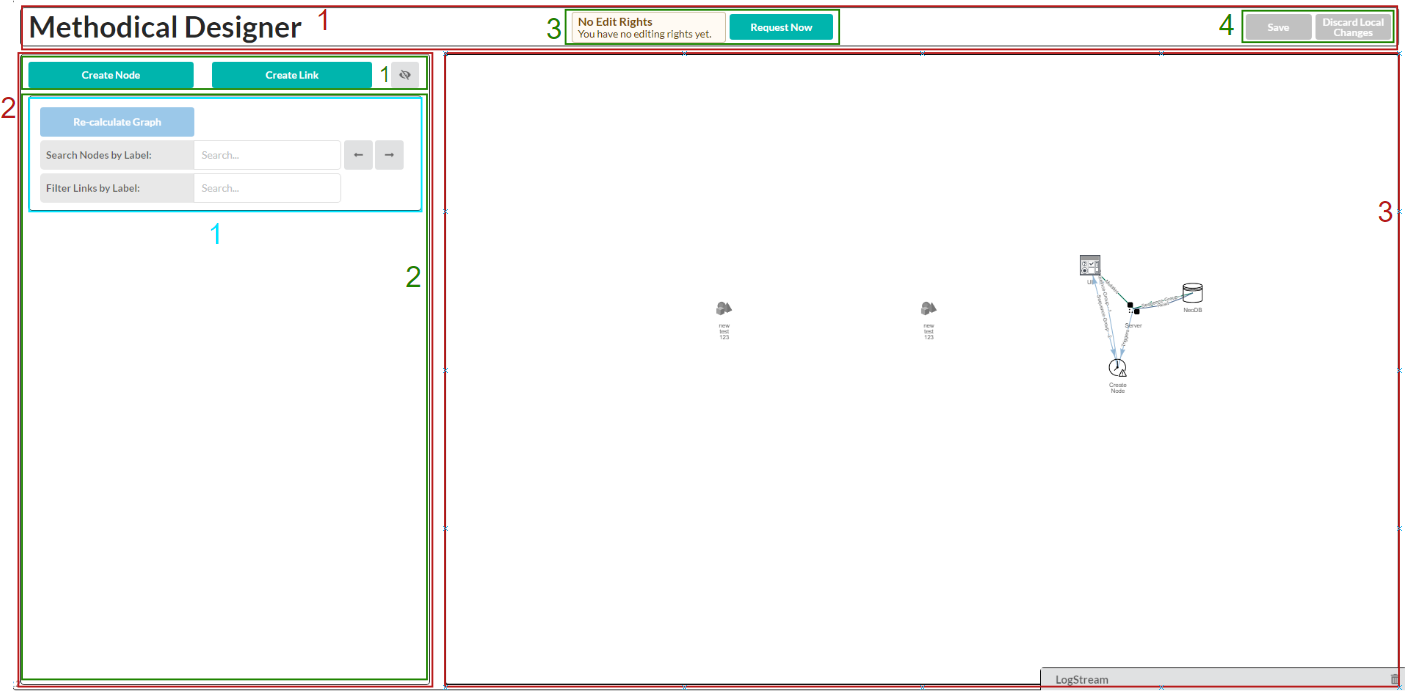
\includegraphics[scale=.46]{Bilder/Layout.png}
\captionof{figure}{The Components in the UI}
\end{figure}
The top level components in red are:
\begin{itemize}
\item[1] \textbf{HeaderArea:} It is almost completely static and contains the name of the application, together with two other components that manage the communication with the server.
\item[2] \textbf{InteractionPane} All components that are required to modify the data of the application will go in here.
\item[3] \textbf{EditorPane} The canvas that contains the graph the user sees.
\end{itemize}

Their child components in green:
\begin{itemize}
\item[1] \textbf{OptionBar} It contains the buttons to create a node or a link, together with a button that will hide the entire \emph{InteractionPane} to give the \emph{EditorPane} the full window width.
\item[2] \textbf{InputPane} All components that require input from the user are child components of this one. This could be called a container component as it doesn't display anything on its own.
\item[3] \textbf{ProjectStatus} Shows information about if the user can make changes to the data and allows the request of editing rights to do so.
\item[4] \textbf{SavePane} Will send changed entities to the server and inform the user about the progress or discard local changes.
\end{itemize}

The child component of the \emph{InputPane} in cyan is called \textbf{GraphSettingsPane}. In the future there will be more options on manipulating data shown in the graph, like filtering for certain types, special layout algorithms etc. What component is displayed here varies depending on what the user last clicked. There are 2 more forms for creating and editing a node or a link.

\section{Problems}
This section will talk about difficulties or problems that appeared during development. For some of them there was a solution found, others are simply to document them for future consideration.

\subsection{Keeping the data consistent when saving changes}
In the very beginning the process of saving local changes to the database was the following: Go through all created/edited/deleted entities and for each of them dispatch a call to the server. This often led to inconsistent data sets that could not be displayed by visjs. To explain this problem consider these few examples of saving scenarios:
\begin{itemize}
\item[1] The user creates 2 nodes and connects them with a link.

Despite this being a very simple example, the approach to save data in Neo4j can cause problems. When creating the link it will look for the IDs of both nodes to connect to. But if for example one of the calls to the database to create the nodes hasn't arrived or wasn't processed yet? Neo4j will throw an error because it is being told to work with a node that doesn't exist.

\item[2] The user deletes a node that has a circular link (both ends of the link point to the same node) attached to it.

Deleting such a node will also automatically lead to the deletion of the link. When the call to delete the node gets processed first, Neo4j will also throw an error as it doesn't allow to delete nodes with relationships.

\item[3] The user deletes a link that has a sequence and link-end property.

As discussed previously, these two exist as their own nodes in Neo4j. Simply deleting the link won't work as it has connected relationships. Using \emph{DETACH DELETE} to delete the node will at least not throw an error, but leave the sequence- and link-end-node fly around in the database with no references. They will not be deleted unless the database is inspected and garbage collected using other tools.
\end{itemize}

There are many more cases where the execution order of queries is critical for keeping the database clean and there might be multiple ways of doing so. At the moment the application makes use of the ES6 function \emph{Promise.all()}. There is an array for each type of operation (creating node, creating link, deleting node, etc.). When the application finds an entity that needs to be sent to the server it will push the return value from the Apollo mutation hook into the respective array. Using \emph{Promise.all( iterable )} it waits for all promises of that type to resolve and only if that is the case it will continue the saving process.

The order used at the moment is the following:
\begin{itemize}
\item[1.] \textbf{Creating and updating nodes} First make sure that all nodes that might be needed later are created. In addition to that any updates made to other nodes can be done simultaneously as that won't affect other entities.
\item[2.] \textbf{Create Links} Add any new links to the database as they might be referenced in sequence- and link-end-creations in the next step.
\item[3.] \textbf{Sequences and Link-Ends} must be created on newly created links
\item[4.] \textbf{Update Links} Changes to Links can be commited safely to the database as any new node they might connect to is guaranteed to exist and internal updates won't affect other entities. In the same step their link-end- and sequence-properties can be updated.
%CHECK IF THIS IS TRUE
\item[5.] \textbf{Delete Links} Remove deleted links from the database. This must be done before deleting nodes as otherwise deleting a node might not work if it has attached relationships.
\item[6.] \textbf{Delete Nodes} Remove deleted nodes from the database. Its important to do this using \emph{DELETE} and not \emph{DETACH DELETE} to make sure there won't be any links without node on one end.
\item[7.] \textbf{Reset Local Store} After that mark all items in the local store as up do date.
\end{itemize}

This code demonstrates the usage of \emph{Promise.all()} to make it more understandable:
\begin{lstlisting}[caption={Usage of Promise.all()}]
for ( let node of createdNodes ) {
	const { id, label, story, synchronous, nodeType, unreliable } = node;
	const variables = { id, label, nodeType, props: { story, synchronous, unreliable } };
	nodePromises.push( runCreateNode( { variables } ) );
}
for ( let node of editedNodes ) {
	const { id, label, story, synchronous, nodeType, unreliable } = node;
	const variables = { id, props: { label, nodeType, story, synchronous, unreliable } };
	nodePromises.push( runUpdateNode( { variables } ) );
}

Promise.all( nodePromises ) 
	.then( () => {
				for ( let link of createdLinks ) {
					...
					createLinkPromises.push( runCreateLink( { variables } ) );				
				}
				Promise.all( createLinkPromises )
					.then( () => {	
		...
\end{lstlisting}
In line 4 and 9 the node promises are pushed into the respective array. All of them are executed instantly. The \emph{then} branch of \emph{Promise.all()} in line 13 will only be reached if all of the promises in \emph{nodePromises} resolve. If that is the case, the mutations to create links can be run, which will also be saved in their array. Once those are resolved the next entity as mentioned above will be handled, etc.

\subsection{AWS-Healthcheck}
After deploying the backend to AWS ECS there was a problem that the server would often be down and couldn't be reached by the application. After looking at the event logs it turned out that the service would restart the task every 3 to 5 minutes due to failed \emph{Health Checks}. These ping a specified URL and compare the response to a pre-defined one. If the response should fail a certain amount of times to be equal to the one defined the service will restart the task as it assumes the task to be stopped, hung or broken in some other way. This lead to a really high CPU usage by the cluster and service and even worse, to the server not being reachable at any moment.

Despite adjusting the settings for the health checks various times to ping the correct route the check would still fail with an error code of \emph{404 Not Found}. In the end the only workaround without having to spend too much time on AWS was to set the code deemed as successful to 404. While this is definitely not a best practice solution it solved the problem in this case. The server ran perfectly and CPU usage by cluster and service dropped significantly:
\begin{figure}[H]
\centering
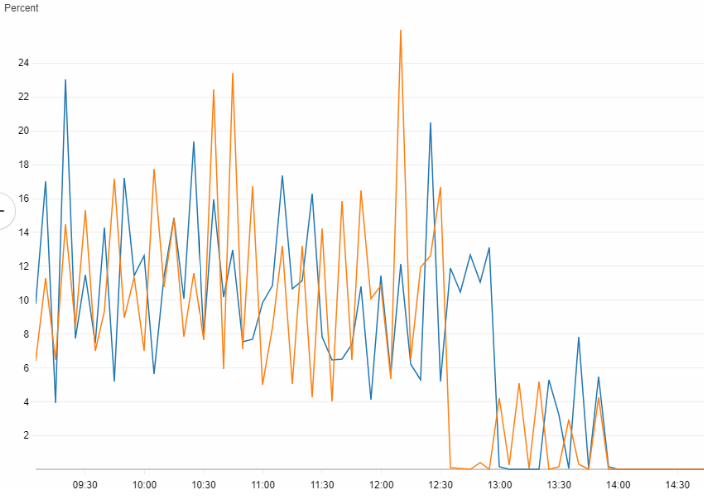
\includegraphics[scale=.6]{Bilder/AwsCpuReduction.png}
\captionof{figure}{CPU Utilization in Percent of Service and Cluster}
\end{figure}

\subsection{Apollo Error-Codes}
When writing the code to curve multiple links between two nodes a first version used the node data from the local cache to iterate through them and find connected links in the links array. While it worked perfectly on the local setup and \emph{most} of the time in the deployed versions, sometimes there appeared an error message: \\

\centerline{Error in setLinks: Invariant Violation: 50 (see https://...)} 

While this message contains something that is similar to an error code, it turned out that these change with every new update to the ApolloClient. This makes it hard to find help online as people who might have had the similar error code probably got it for a different reason. At some point the error also appeared on the local setup and there the ApolloClient serves an error message with a lot more information. 

As it turned out, the source of the problem was that in the code to calculate the custom curvature reading the nodes from the cache would sometimes end in an error if the query for nodes hasn't returned data yet. However instead of returning undefined - which would have led to a typical JavaScript error that is easy to track down - Apollo throws an error itself. The reason for a different message between production and development environments is that in production environments Apollo strips these error messages to a minimum to reduce the bundle size. \\

The solution to getting error messages with more information even in a production environment was to write a few wrapper methods that take a GraphQL query, the data to write into the cache and an error string that gets printed in case something goes wrong.

\subsection{Apollo Chrome Dev-Tools}
As often said, Apollo is a great tool and it offers a lot of functionality. Debugging however was not such a pleasant experience as the Dev Tools seemed to have only around a 50\% chance of being able to connect to the application:
\begin{figure}[H]
\centering

\includegraphics[scale=.65]{Bilder/ScreenOfDeath.png}
\captionof{figure}{The Apollo Dev Tools can't connect}
\end{figure}
This became especially annoying when wanting to check the local state after completing certain steps and then having to re-load the page a few times.

\subsection{CORS-problems}
Something very useful when using AWS Amplify is that when creating a web app with it, marking the URL in the address bar as secure which makes the application appear more serious.

But it comes with one problem. Amplify configures its applications in a way that it only accepts data from other resources marked as secure. As the backend did not have a certificate at that point any communication would be blocked by Amplify resulting in a CORS-error. \\

So what exactly is CORS? It stands from \emph{Cross-origin resource sharing} and is a way to configure websites to accept data requested from another domain than their own. \\

Even after spending a lot of time searching for a setting to disable this behavior from Amplify and configuring the ApolloClient according to the docs to allow CORS to make sure its not a configuration problem from the application, the results stayed the same.

The only remedy to this issue was to get a certificate for the backend and by that mark it as a secure resource. After that all communication worked without any issues.

\newpage
\section{Graph-Layout}
As mentioned in the introduction, the ability to create a graph on its own is a central aspect of the application. This part offers a lot of room for improvement as graph layout is its own field of research and the algorithms can become incredibly complex. Here are two approaches described together with their flaws and benefits.

One main problem both tries face is that in order to allocate them, a start-node must be found that the others can use to orientate themselves on. But which node should be chosen to start? The one with the most connections? Where should nodes that are not children of the start-node be placed? 

Nodes that can be collapsed (hide their direct descendant children) are placed in a grid-like manner. Then their children are placed relatively to them. After handling all child-nodes, the ones that were not part of a collapsable were handled. For those the ones with the most connections would be chosen as start-node.

\subsection{Tree-Layout}
In this approach each node would distribute its child nodes below it. Depending on the amount of children they'd be split into different layers of nodes.

While the tree logic was relatively easy to implement and created at least acceptable images as seen in \autoref{ex:TreeGood}, it had a lot of flaws with the biggest one being overlapping edges or edges that move through the middle of nodes making it impossible to see the actual connections like in \autoref{ex:TreeBadEdge}.

\begin{figure}[H]
\centering
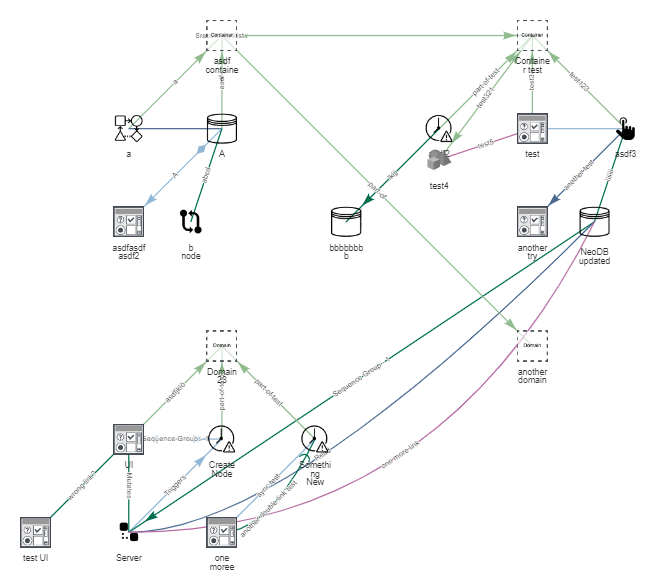
\includegraphics[scale=.7]{Bilder/TreeGood.png}
\captionof{figure}{Layout created by the Tree Algorithm}
\label{ex:TreeGood}
\end{figure}

\begin{figure}[H] 
\centering
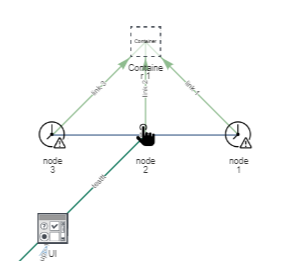
\includegraphics[scale=.4]{Bilder/TreeBad.png}
\caption{Edge moving directly through Node}
\label{ex:TreeBadEdge}
\end{figure}

Furthermore if the trees grow very long they'll sooner or later intersect with each other. One option would be to iterate over all previously placed nodes and check their positions before placing another one and by that define an offset to the deepest one. However the performance would most likely make the app unusable once the graph becomes larger.

\subsection{Flower-Layout}
The name for this layout comes from the idea of creating flower shaped groups of nodes. The basic idea is to select one center-node as described above and place its direct descendants equally around it it creates a circular shape. Child-nodes of these descendants then use the direction vector of their parents link to place themselves accordingly.

\begin{figure}[H]
\centering
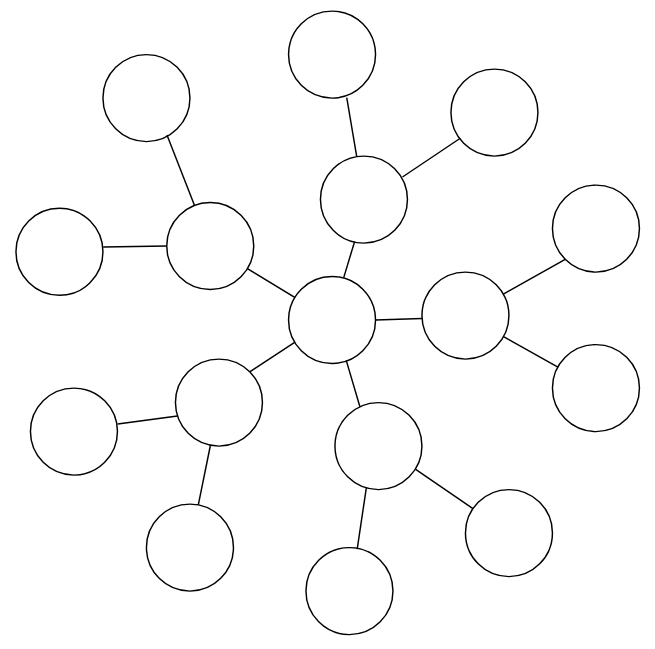
\includegraphics[scale=.55]{Bilder/FlowerEx.png}
\captionof{figure}{Basic Idea of the Flower Layout}
\end{figure}

This algorithm uses the available space a lot better and as it grows into all directions overlapping with other groups becomes less likely. Furthermore there are many parameters that can be adjusted. For example the distance to the parent-node can depend on the amount of child-nodes the current node itself has:

\begin{figure}[H]
\centering
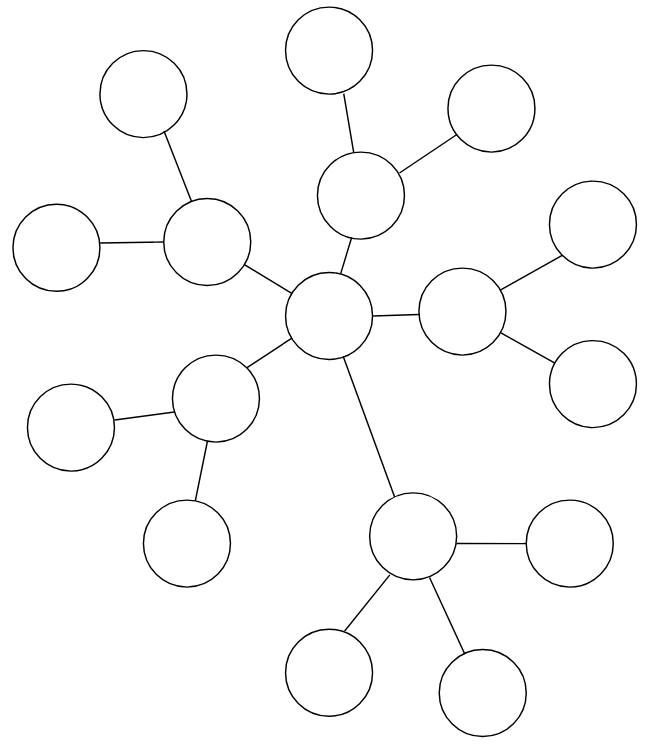
\includegraphics[scale=.4]{Bilder/FlowerDistEx.png}
\captionof{figure}{Node with more Children is further away}
\end{figure}

While this approach sounds promising it of course also has flaws. To demonstrate those lets look at an example from testing data and explain whats happening:

\begin{figure}[H]
\label{ex:TreeBad}
\centering
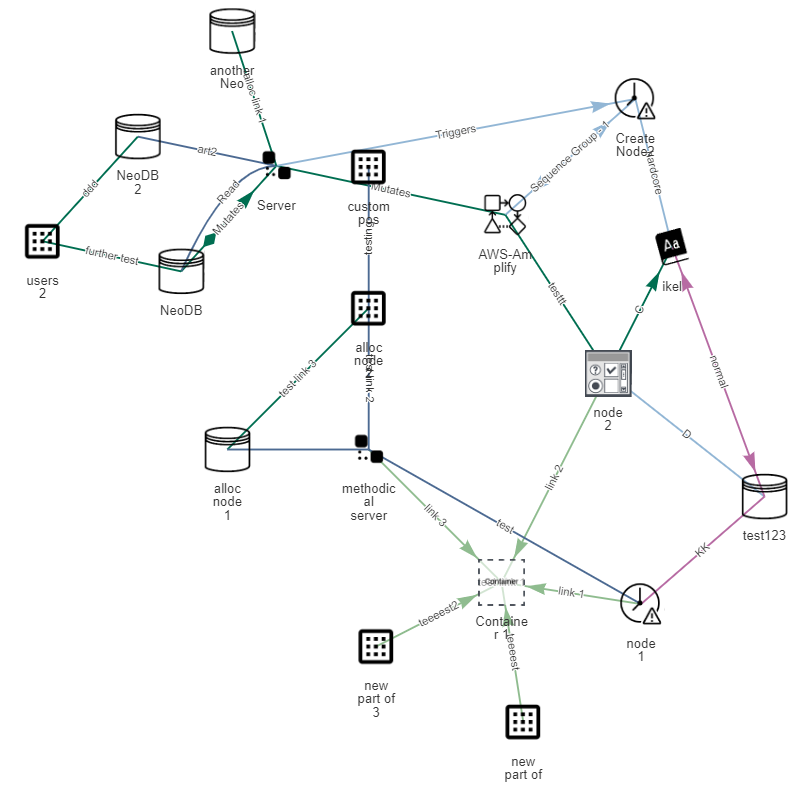
\includegraphics[scale=.55]{Bilder/FlowerExBad.png}
\captionof{figure}{Intersections in the Flower Layout}
\end{figure}

The container on the bottom is selected as "Center" as it is a collapsable. Its child nodes are distributed around it by equally sized angles. Its also clearly visible that the nodes \emph{node 2} and \emph{methodical server} have a greater distance to their parent-node than the other 3 as they have zero or 1 child element.

As \emph{test123} is a child of both \emph{node 2} and \emph{node 1} it takes into account two direction vectors: One from \emph{Container 1} to \emph{node 1} and the one it gets assigned from \emph{node 2}. Every node will allocate its child nodes within an angle of +-90° to its own direction vector. These two vectors get divided in two and the result will lead to the position of \emph{test123}. The reason for \emph{Server} being so far away from \emph{AWS-Amplify} is because it has 3 child-nodes.

Now to the flaws of this approach: The node in the top center intersects with other, not related links. The reason for that is that as it is the only child element, it will simply extend its parents direction vector.
In addition there are many more places where nodes or links could intersect. Also, if one or more nodes have a connection to another group of nodes, they might be placed very far from each other and their connections could intersect with many others.

As this approach in many cases lead to more promising results than the tree layout algorithm it is the one currently in use. This can be seen by directly comparing its result to the Tree Layout with the same data as in \autoref{ex:TreeGood}:

\begin{figure}[H]
\centering
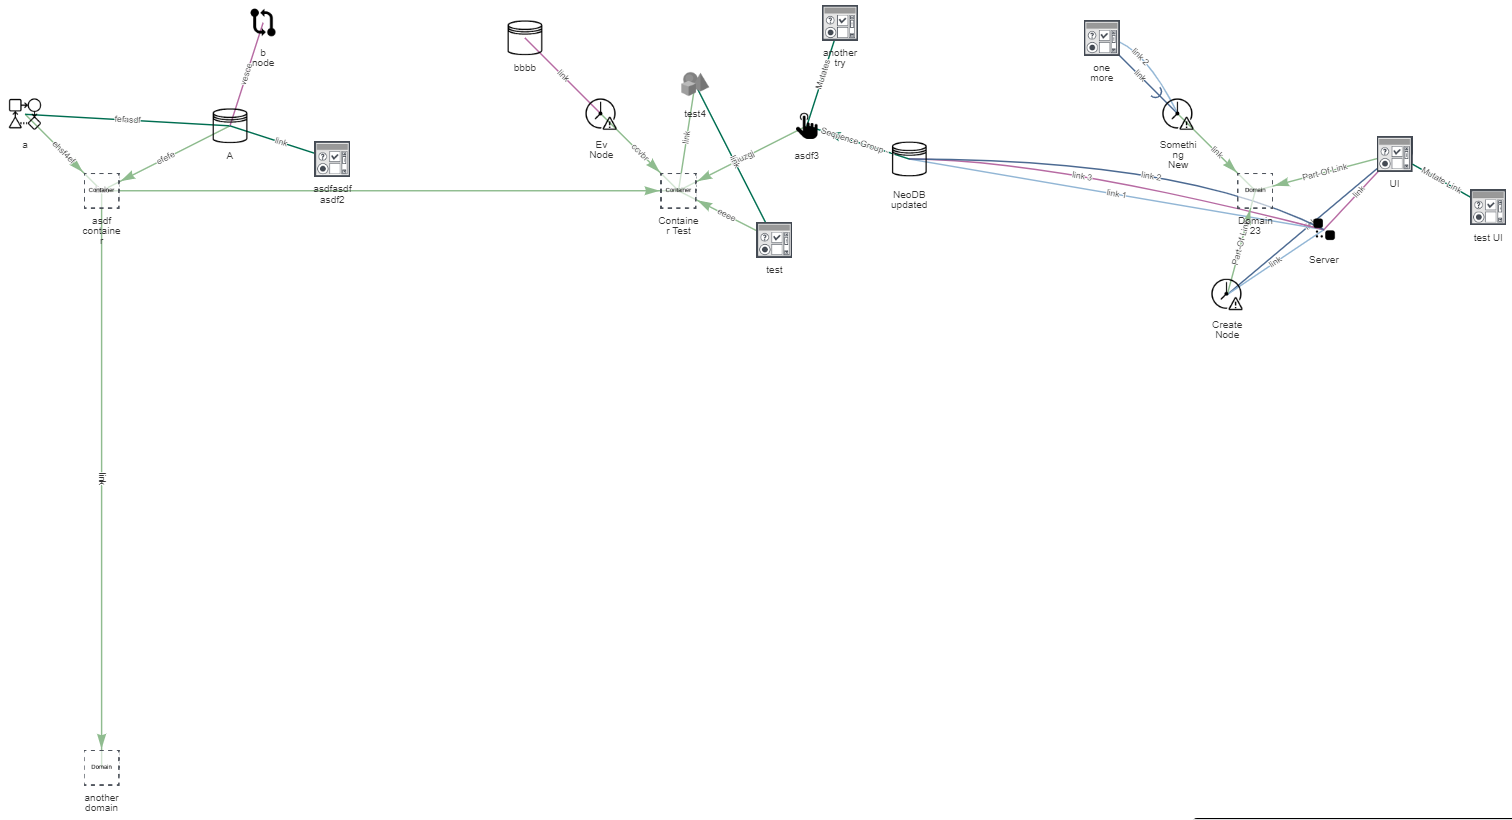
\includegraphics[scale=.4]{Bilder/FlowerCompTree.png}
\captionof{figure}{Layout Created by Flower Algorithm}
\label{ex:ComparisonTreeFlower}
\end{figure}

\newpage
\section{Behavior Decisions}
When implementing the user interface and the inner logic of the application there will often be the question \emph{How should the application behave if ...?}. Here are some that appeared in this project together with some ideas on what options were available:
\begin{itemize}
\item What should happen when a node that has links connected gets deleted? As visjs doesn't offer the option of simply leaving the link there, solutions similar to the following have to be considered:
\begin{itemize}
\item Deleting a node with connected links is not possible.
\item The connected links snap to the node thats closest by.
\item Each link snaps to the other node it is connected to, creating a circle.
\end{itemize}
In the end number 3 got implemented as it is the most usable and predictable behavior for this use case.

\item What should happen if a \emph{Part-Of} link connects two collapsables and the user clicks \emph{Collapse} on one of them?
\begin{itemize}
\item Both collapsables should disappear together with their child-nodes.
\item If the collapsable that issues the collapse call is the parent in the connection, the other one disappears. Otherwise both stay visible.
\item The creation of such connections should not be possible.
\end{itemize}
In this case the second option got implemented as number 1 would make the application not usable and the third one might limit the user in the use of the application.

To demonstrate this, lets take a look at this picture:
\begin{figure}[H]
\centering
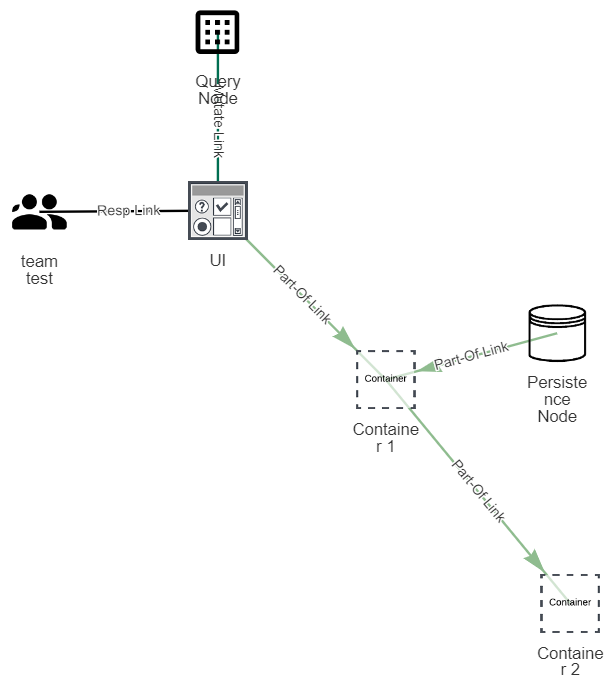
\includegraphics[scale=.55]{Bilder/CollapseExBefore.png}
\captionof{figure}{Two Collapsables Connected Through a Part-Of link. \emph{Container 1} is the child of \emph{Container 2}}
\end{figure}

If the user clicks \emph{Collapse} on \emph{Container 1} the image will change to the following:
\begin{figure}[H]
\centering
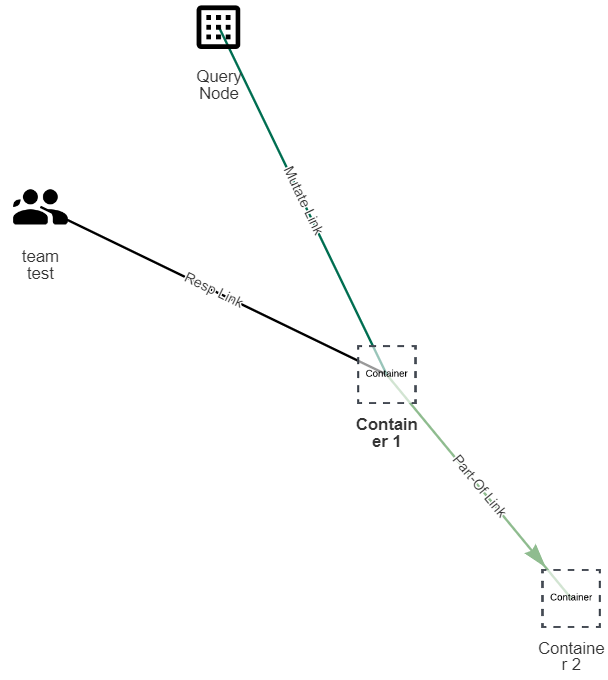
\includegraphics[scale=.55]{Bilder/CollapseExAfter.png}
\captionof{figure}{The child nodes of \emph{Container 1} disappeared. \emph{Container 2} is still visible as it is defined as parent in the link connecting the two containers.}
\end{figure}

\item How is a part-of relationship defined? In other words, which nodes should disappear if a collapsable gets collapsed?
\begin{itemize}
\item All nodes that the flower layout identifies as children of a collapsable.
\item Only nodes with a direct part-of link to the collapsable will disappear
\end{itemize}
The second options was the one to go for, as in the first one it is almost impossible to algorithmically detect which node should be the last one to disappear if the user created connections between groups created by the flower layout algorithm. Nodes that are not part of the current group might disappear as well.
\end{itemize}

\newpage
\section{Avoiding Data Corruption}
After deploying the application a problem that hasn't appeared before suddenly came up: As there is no user logic yet and only one dataset, what happens if two people open the app at the same time and make changes to the data that are not compatible? Just imagine user 1 deleting a node in his editor, while user 2 creates a new link to that node. When merging these changes the database will most likely run into an error case and abort the commits.

To avoid scenarios like this the user can't actually make changes right away when opening the app. Instead he has to request editing rights by clicking a button at the top of the screen. Should someone else have requested rights before he'll receive a message telling him so. Otherwise the app will sync with the database to fetch the latest changes and allow changes to the local dataset.

This is implemented by having a \emph{project} node in Neo4j that contains a property called \emph{isBeingEdited}. When requesting the editing rights the server will fetch the node and check the value of this property. Should it be true the server will return false as in requesting editing rights was not successful. Otherwise it'll set the property to true and then return true to indicate a successful operation.

\chapter{Looking back}
\label{chap:LB}
This chapter will shorty list some things that were positive in this project and then also others that weren't ideal.

\section{What was good}
\begin{itemize}
\item \textbf{It works!} Despite many problems especially with Apollo and the configuration during the deployment phase the application works and runs stable on a publicly shared cloud platform without any known bugs in the functionality which is a big success. Deploying as early as possible allowed others to use and test the system from an early stage on an provide valuable feedback during development.

\item \textbf{Interesting} Learning all of the technologies from scratch at the beginning of the project was of course a lot to take in. But with time came more understanding of every part and it was interesting to take a deep dive into this area of software development and get to explore profoundly all parts of it.
\end{itemize}

\section{What was not ideal}
\begin{itemize}
\item \textbf{Warmup time} Trying to get going as quickly as possible right in the beginning was not best choice. The reason for doing so was to have something to show to others early in the development and to avoid having time issues later on. However it might have turned out to be quicker to first get a good overview of all the technologies and frameworks, especially Apollo. It offers a lot of functionality and taking more time in the beginning could have been faster and led to a cleaner code base in the end.

\item \textbf{Apollo} Despite having said that it is a great frameworks and offers a lot of functionality it would probably have been better to go without it. It is a very big dependency and a lot to take in, but the app only makes use of very small and specific parts of it, the most important one being state management. While it is not bad at it there is no big advantage of it over using a pure state management library like Redux. Furthermore having to define a GraphQL query for fetching the local state creates many lines of code and the queries all ended up being almost similar which invalidates the argument of getting only the needed data. In addition to that it made development slower because many times it later turned out that another property, or even a few which have to be added to the query, are needed in a mutation. In the end queries often end up being so similar that the only logical thing would be to use the same query for many different purposes.

While Apollo is the first result when looking for \emph{How to create a GraphQL server} in Google it is not the only way and if in the beginning only small subsets of Apollo's functionality is needed it is most likely the wrong choice.
\end{itemize}


\chapter{Ideas for the Future}
\label{chap:Future}
This part contains a list of ideas about what could be added or modified in the project in possible further development together with some suggestions on how these could be approached.
\begin{itemize}
\item \textbf{UI/UX} improvements to make working with the application more comfortable.
\begin{itemize}
\item The \textbf{responsiveness} of the website. Maybe even re-creating the structure of the app using a mobile-first approach might be a good idea, otherwise adapting the css values would be the way to go.

\item \textbf{Undo-redo} logic by using the command pattern. This can be added gradually for one action at a time. A good thing to start with might be the creation of nodes and links. Whenever the user completes such an action it gets added to a history object in the cache, containing the ID of the created item. Should the user then presses Ctrl+Z or clicks an undo button the item gets removed from the cache and the action from the history object.

\item \textbf{Context actions} to create nodes and links by using the visjs \emph{oncontext} event and displaying a form on the screen at the position clicked. The coordinates can be extracted from the event object passed into the event handler.
\end{itemize}

\item A \textbf{Syntax Checker} for connections between nodes. The app doesn't put any restrictions on the creation of links. This is on purpose as specific use cases might require combinations that can't be foreseen when creating the app. However displaying warnings for certain combinations can be of very high value and make the user aware of structures that he didn't mean to create. In general this should be done using web workers as checking all connections could take a lot of time, depending on number and complexity of the rules and the amount of connections in the diagram. At first only single links should be the focus, later on whole constructs could be checked. Rules to start with could be:
\begin{itemize}
\item Collapsables can only have \emph{Part-Of} links
\item Loops between collapsables
\item Only \emph{Team} nodes can have \emph{Responsibility} links
\end{itemize}

\item Allow the user to define \textbf{Custom Rules} for the syntax checker. This would be a very big task as it involves the definition of some abstract language and a parser that can convert these into constructs the syntax checking algorithm can use.

\item Allow the user to define \textbf{Custom Types} of nodes and links. This and the previous point require implementing a way of uploading and saving these definitions in the application.

\item \textbf{Improve Layout Algorithm} to create a better looking image. Two ideas are
\begin{itemize}
\item A \textbf{distance system} that when calculating the position for a node first checks if this new place is close to other already placed nodes. If it is closer than a certain number the algorithm will search for a new position. The minimum distance can vary depending on the type of the node.
\item Place \textbf{connected nodes} closer to each other. Connections could receive a weight and "pull" heavily connected nodes closer to each other.
\end{itemize}

\item \textbf{Subscriptions} to allow users to get real time updates to changes made to the data. Using a button the user could activate and deactivate the feature. This functionality could be implemented using the pubsub npm package, as recommended by Apollo.

\item \textbf{User/Project Logic} to make the app usable for a broader amount of people. It would be enough to have a simple login screen when the app starts. Once successfully logged in there is a list of projects the user can choose from. Projects and users could be associated through respective nodes. One node per user and each user node could be connected to a variety of project nodes which in term again are connected to nodes that are part of it. This could lead to the database getting blown up quickly so it might be a good idea to create a new database every time a user signs up.

\item \textbf{Refactor} the codebase.
\begin{itemize}
\item Starting with the GraphQL schema and removing the input types would make the preparation for dispatches to the database a lot cleaner. 
\item Abstracting the input logic would allow to extract it into a React HOC and take a lot of code out of the forms used for creating and editing nodes and links.
\item Shortly after the development phase of this project finished Apollo completely released the Apollo Client 3. Upgrading and making the whole project conform to the documentation and recommendations of Apollo would make the codebase cleaner.
\item One might even consider to get rid of Apollo entirely and build the project using Redux, Neo4j, React and purely the \emph{graphql} npm package.
\item A lot of the state management logic can be shortened if initially a graph like datastructure would be built and saved in the cache instead of sticking to a list of nodes that have a list of IDs they are connected to.
\end{itemize}

\item \textbf{Improve Collapsables} to increase the value they have to make the graphs cleaner. \autoref{ex:CollExpanded} shows how collapsables could look at some point when being expanded while \autoref{ex:CollColapsed} demonstrated a collapsed one.

Implementing this in visjs might not be the most enjoyable task as it does not natively offer functionality to draw a rectangle around a group of elements.

One way would be to get the position of all part-of elements, calculate the middle of them and get the outer bounding box measurements to define the size of the box. 

\item \textbf{Versioning} with Git to be able to version graphs to track changes or export them to create backups. This would require to define an algorithm that can convert graph data into for example JSON or XML files. These files could then be stored in GitHub. 

\item \textbf{References} to other diagrams or items of the same diagram. 
It often happens that structures appear various times in project architecture. This functionality would apply changes made to one of them to all copies of the other in the current diagram.

If a user has various diagrams it'd be useful if he could create a node that links to other diagrams and by clicking on them they open up in a new tab of the screen. 
\end{itemize}

\begin{figure}[h]
\centering
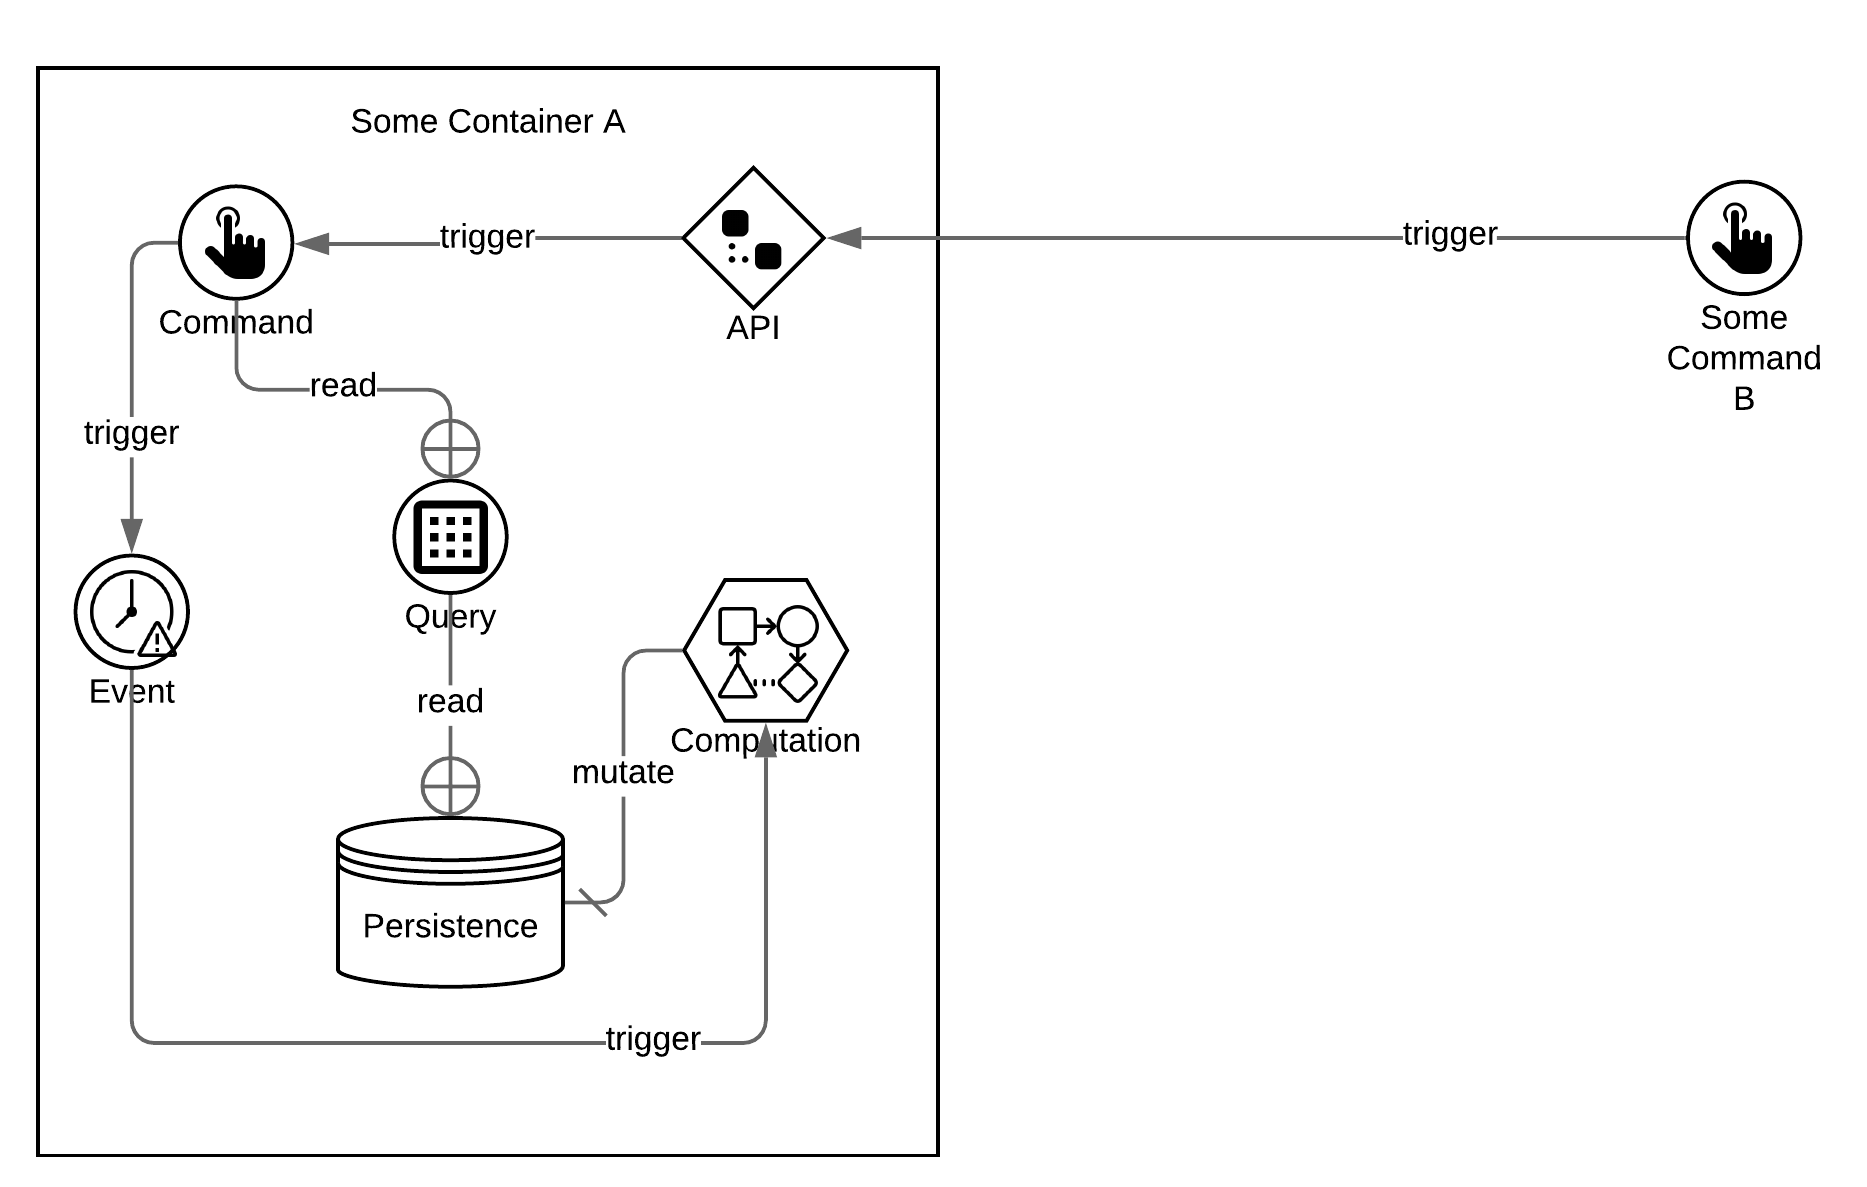
\includegraphics[scale=.35]{Bilder/CollapsableEx.png}
\captionof{figure}{Example Collapsable in Expanded State}
\label{ex:CollExpanded}

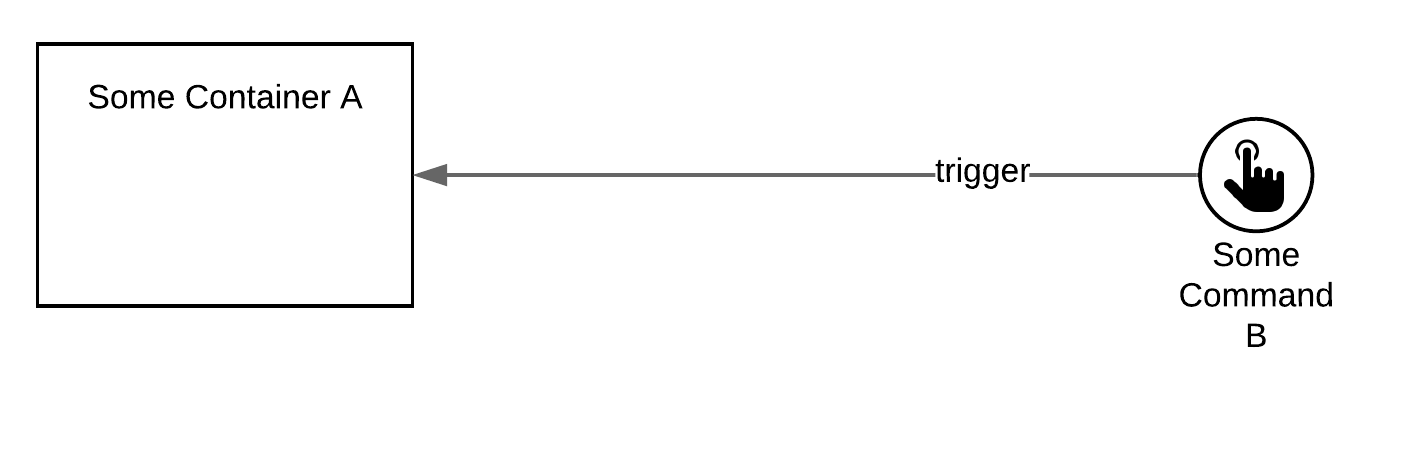
\includegraphics[scale=.4]{Bilder/CollapsableCol.png}
\captionof{figure}{Example Collapsable in Collapsed State}
\label{ex:CollColapsed}
\end{figure}

\chapter{Documentation}
\label{chap:Doc}
This section will explain how to set up a local environment, as well as a short walk-through through the codebase.

\section{Setting Up a Local Development Environment}
\subsection{Neo4j Desktop}
\label{chap:NeoDesktop}
Download Neo4j Desktop from the official Neo4j download page \cite{NeoDownload} and install it. After the installation process start the application and enter the activation key from the download page.
Create a new project by clicking \emph{New}. When clicking on \emph{Add Database} choose the option \emph{Create a Local Database}. Its important to write down the password as it is necessary to connect to the database. The version used while writing this is 4.1.0. Click on \emph{Create} and wait for the process to finish.
Then under \emph{Plugins} click \emph{Add Plugin}, choose \emph{APOC}, confirm the installation for all graphs and close the window. The window should look similar to this:
\begin{figure}[H]
\centering
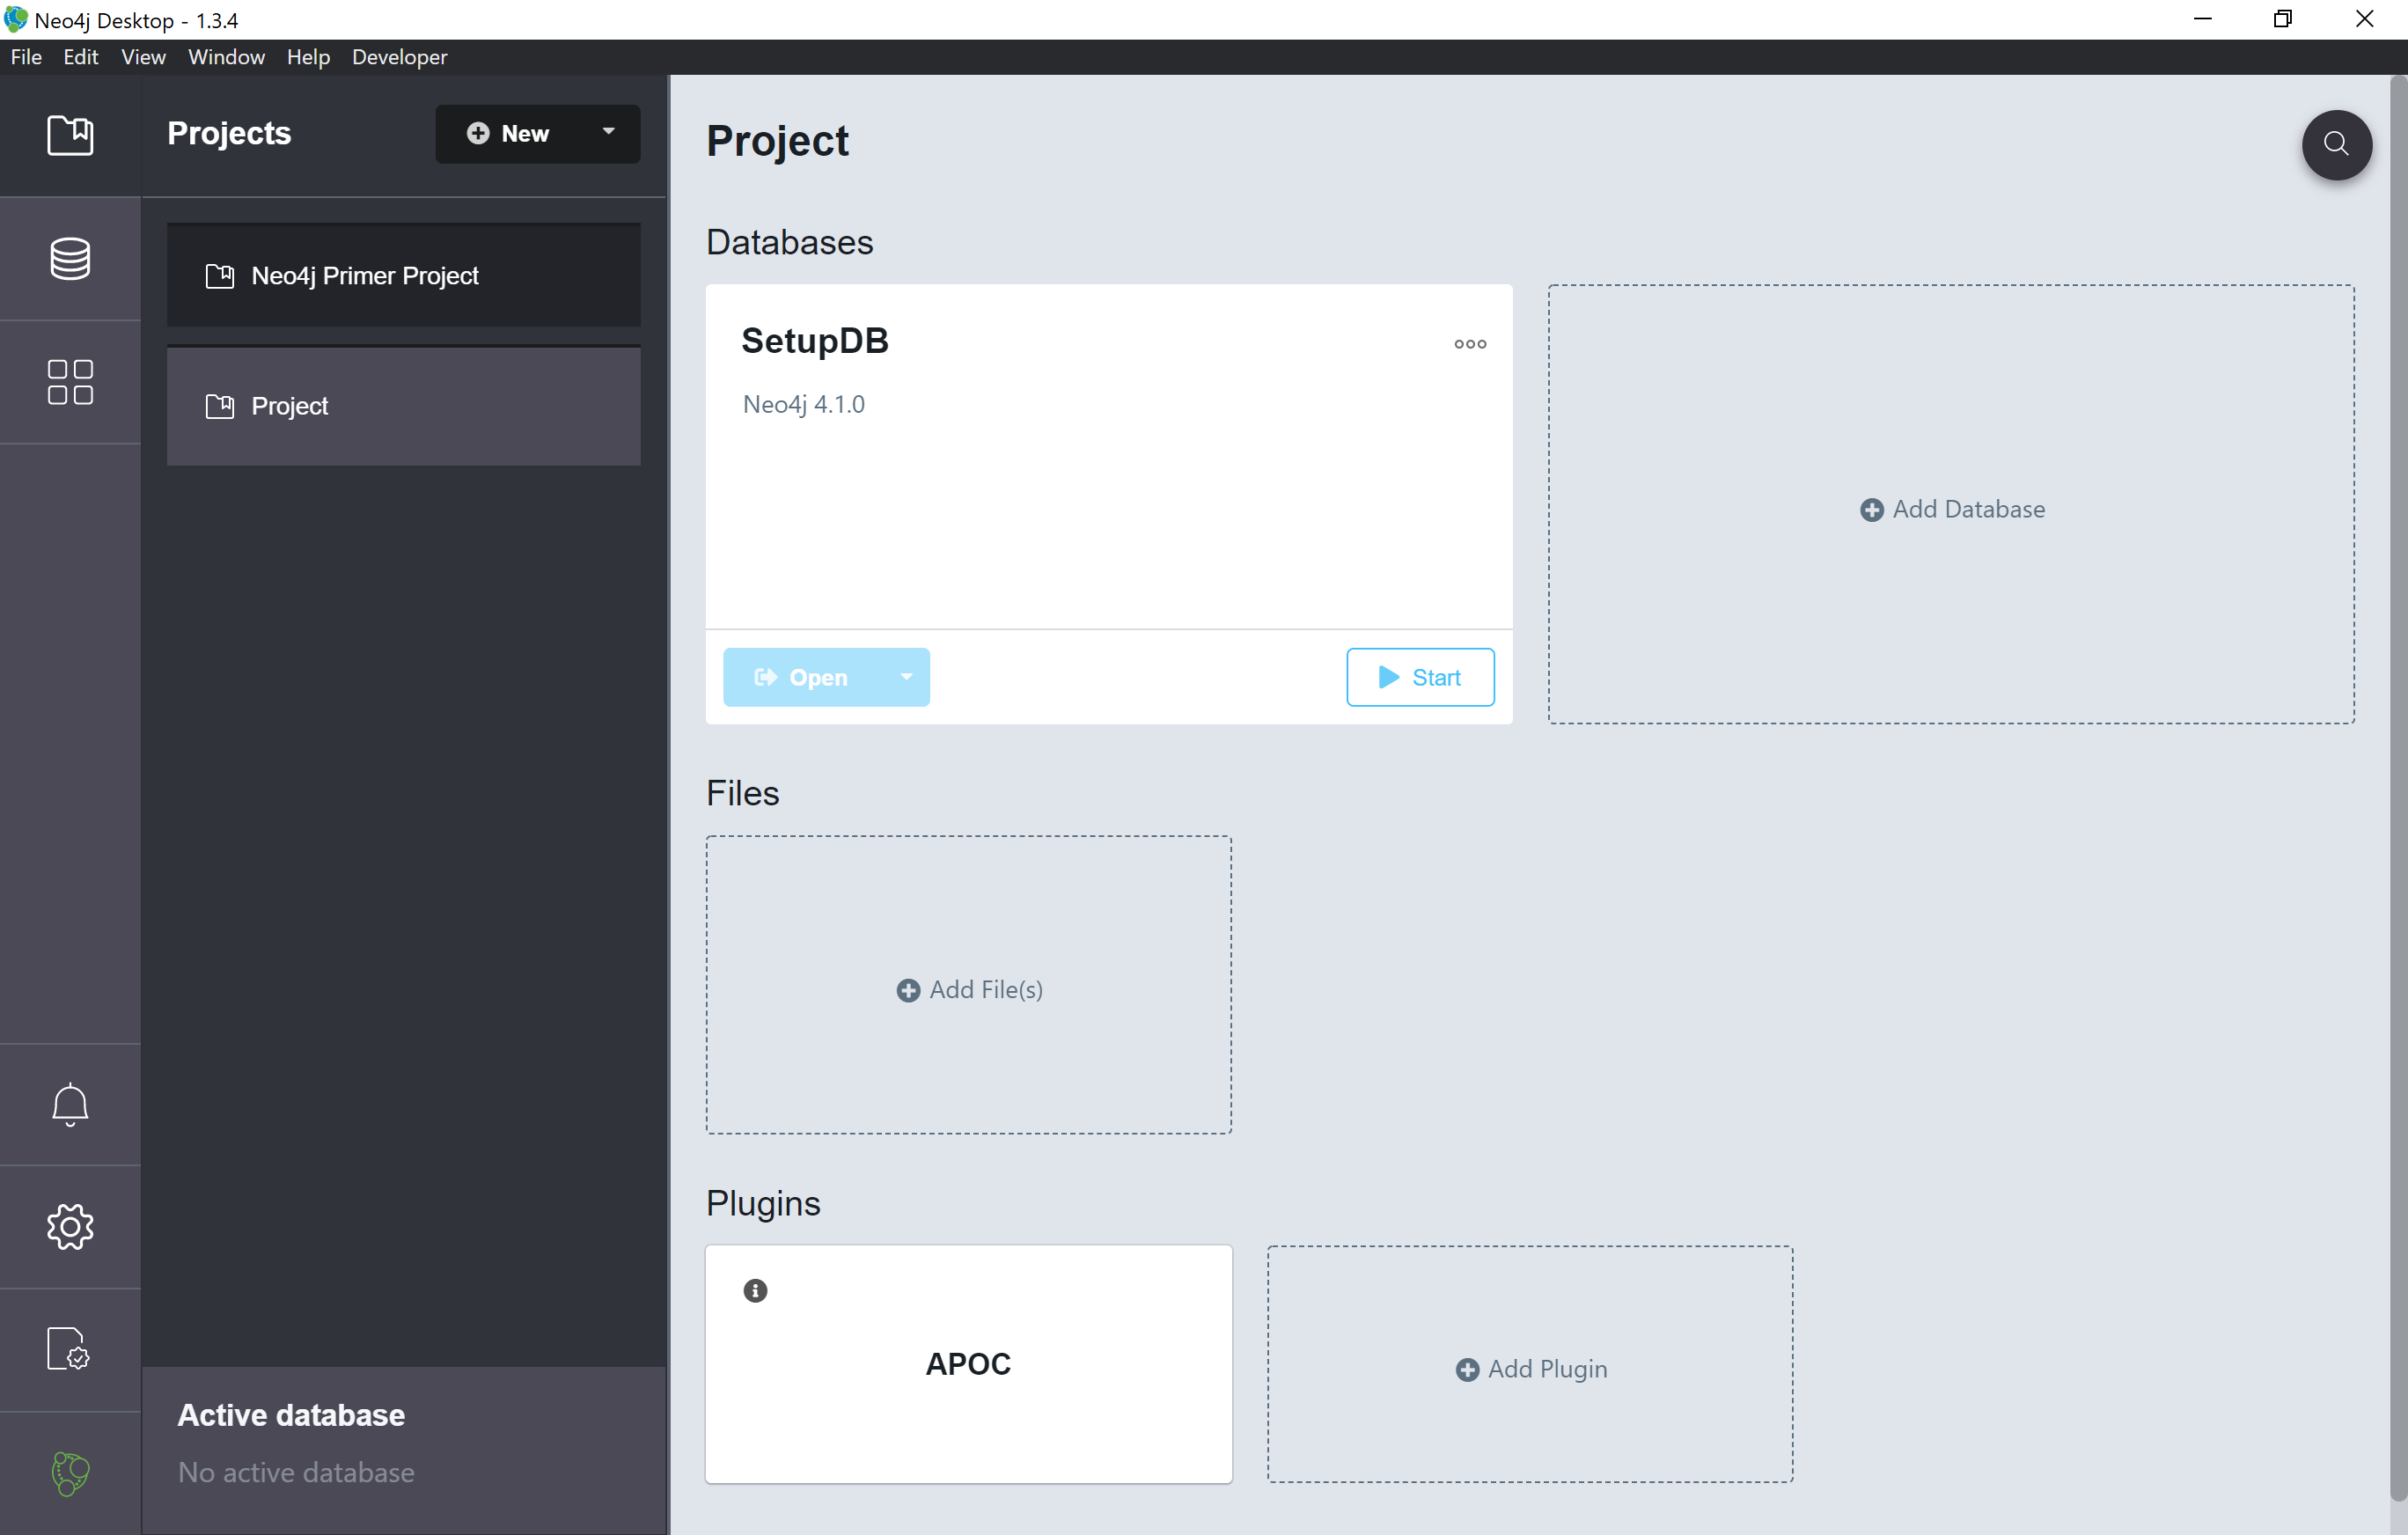
\includegraphics[scale=.4]{Bilder/NeoDesktopInit.png}
\captionof{figure}{Neo4j Desktop after Creating the Database}
\label{ex:NeoDesktop}
\end{figure}

Next hit \emph{Start} to spin up the instance. When it is running click on \emph{Open} to start the Neo4j Browser. In this browser all Cypher queries can be executed directly on the database.

\newpage
\subsection{Creating a Project Node}
In order to be able to request editing rights and actually use the app, it is necessary to manually create a project node in the Neo4j Browser that contains a property called \emph{isBeingEdited} set to \emph{false}:
\lstset{language=Cypher}
\begin{lstlisting}[caption={Creating the necessary Project Node}]
CREATE (p:Project {isBeingEdited: false}) RETURN p
\end{lstlisting}

\subsection{Backend}
Install Node.js, clone the server \cite{GitServer} code from GitHub. Open a console window, navigate into the folder containing the server code and execute \emph{npm install}. Inside the server folder, create a file called \emph{.env} with the following content:
\lstset{language=Docker}
\begin{lstlisting}[caption={Environment Variables for the Server}]
PORT=8080
ENDPOINT=/graphql
DB_DEV_PW=<YOUR_DB_PW>
DB_USER=neo4j
DB_DEV_HOST=localhost
DB_PORT=7687
NODE_ENV=development
\end{lstlisting}
This defines the port and path for the GraphQL Playground provided by the server. Furthermore it provides the endpoint where the server can reach the database. The port can be found by clicking on the 3 points on the right of \emph{SetupDB} in \autoref{ex:NeoDesktop} but is \emph{7687} by default. At \emph{DB\_DEV\_PW} make sure to put the password chosen in \autoref{chap:NeoDesktop}.
Now type \emph{npm run start-dev} into the console to spin up the local development server. After loading for a short time the console window should state a message similar to \\
"Server vX.X started at ... listening on http://localhost:8080/graphql" \\
Visiting this URL will open the GraphQL Playground that can be used to test the resolvers of the server for example as shown in \autoref{ex:RunCreateNode}.

\subsection{Frontend}
Clone the client \cite{GitClient} code from GitHub, open a console window, navigate into the client folder and execute \emph{npm install}. In the same folder, create a \emph{.env} file with the following content:
\begin{lstlisting}[caption={Environment Variables for the Frontend}]
REACT_APP_ENV=dev
REACT_APP_DEV_HOST=http://localhost:8080/graphql
\end{lstlisting}
The first variable is used to define the favicon in the browser tab, the second one points to the URL of the server. Then running \emph{npm start} will create a production build with live updates at \emph{localhost:3000}.

\section{Backend}
This section will quickly explain the contents of some of the server files and short explanations where it might be necessary.
\begin{itemize}
\item \textbf{index.js} The app first constructs the neo4j driver to communicate with the database. The required URL is taken from the environment variables. Next up is the creation of the ApolloServer-instance. It receives the neo4j driver in the context and the GraphQL schema. If the \emph{NODE\_ENV} variable is set to \emph{production} the server will deactivate the GraphQL Playground and introspection. This is a feature that allows the server to create a documentation of the queries and types the server offers and make it available in the Playground.

The \emph{errorPlugin} is a small function that prints server errors in a more readable way than it'd be the case without it.

The \emph{exitHandler} function makes sure that any open connections to the database are closed in case of the server shutting down due to an error or any other exit code.

\item \textbf{resolvers.js} Contains all resolvers. To get the result from running a query the \emph{PrepareReturn} function in \emph{ResolverUtils.js} is used. The reason for doing so is that ApolloServer will throw an error if not all fields from a node exist, so the function checks if the fields exist and fills them with dummy data if not.

\item \textbf{graphql-schema.js and schema.graphql} The first file converts the schema file into a string and allows to combine multiple schema files in case it spreads over more than one.

\item \textbf{Dockerfile} These are used to deploy to AWS. They set a base environment and copy necessary data into a docker image and install the packages listed in \emph{package.json}. In the end it defines the necessary environment variables and runs the npm start commands.
\end{itemize}

\section{Frontend}
This part will explain the most important files and parts of the client code.
\begin{itemize}
\item \textbf{ApolloProvider.js} This is the entry point for the application. It defines an \emph{InMemoryCache} that contains typePolicies, which are a way of telling Apollo how to fetch local fields. They are important to make sure the client doesn't return \emph{undefined} for a property if it doesn't exist as it would throw an error.

Furthermore this file contains the local resolver functions inside the \emph{ApolloClient} object. In the end it defines an initial state object.

\item \textbf{App.js} is the parent component for all other displayed on screen. It will fetch all links and nodes from the server. Once they get returned it passes them to a local resolver function to set all fields that are necessary for local state management.

\item \textbf{components} The components folder contains almost all of the React components. \emph{CreateLink, CreateNode} and its counterparts for link entities are the forms dealing with user input. \emph{EditorPane} displays the canvas on screen. It contains queries listening for updates to the camera position, link and node changes, as well as a \emph{createNode} mutation to create nodes when the user presses Ctrl+V.

Below that it contains the definition of visjs events:
\begin{itemize}
\item When the user clicks a link or node that item will be set as active. This will change the form displayed on the left side of the screen and fill it with the data from the entity clicked.
\item  Zoom saves the coordinates the user zoomed to.  In case he creates a new node it will appear at that position. The same counts for \emph{dragEnd} if no node was selected.
\item If a node is selected the new position of it will be saved. If the user presses "recalculate graph" it gets reset.
\item When clicking at a certain location without selecting a node or link the position gets saved for the next node creation.
\end{itemize}

\item \textbf{GraphSettingsPane} contains the fields to search for a node and filter links according to their label.

\item \textbf{LogStream} is a small component that appears on the bottom right of the window. It displays error messages and general information.
\end{itemize}

\subsection{Local Resolvers}
This section will talk in a bit more detail about the more complicated resolvers in \emph{ApolloResolver}. Something very important that counts for all of them is that data read from the cache is immutable and trying to modify it will result in an error. Thats why in most resolver as soon as data was read from the cache the code will create a \emph{deepCopy} of it.

\subsubsection{setNodes, setLinks}
When the nodes and links come from the database for example after the initial fetch or when syncing after requesting editing rights they are missing some data to be usable locally.

To know whether local changes have happened each entity needs the properties \emph{edited, created, deleted}. In addition to that nodes receive a listIndex which makes sure their order does not get changed when making changes as this would lead to unpredictable graph layout updates. Furthermore nodes and links both have a property called \emph{needsCalculation}. If the user changes the nodes a link is connected to or a node changes its type this property gets set to true and the button to recalculate the graph layout becomes clickable.

\subsubsection{updateLink}
This resolver is quite large as each node contains a list of IDs of the nodes it is connected to. If the user changes the connections of a link filtering and updating these lists takes a bit of effort.

The function first gets the current connected nodes. Then it sets the new internal properties of the updated link and compare the IDs of the connected nodes to the ones previous to updating. Should they be different it'll update the previously mentioned lists of connected nodes.

\subsubsection{collapseNode}
When collapsing or expanding a container or domain node the respective property first gets inverted. Afterwards all nodes that are connected through a \emph{Part-Of} link get hidden. This also goes recursively, meaning that if a container has a domain connected via such a link it and its children will also get hidden.

Then, all links that were connected to now hidden nodes will snap to the container that issued the collapse command to visualize that the actual partner node is hidden.

As a last step links that now connect the same nodes as a result of the collapse command get a curvature to make sure they do not lay on top of each other.

\subsubsection{setNodeLabelFilter}
This sets the search string but doesn't actually execute the search. It just saves the value for the search input. Right afterwards the search function gets executed. This could be refactored, see \autoref{chap:Future}.

\subsubsection{searchNodeByLabel}
This function does the actual searching. It uses the \emph{Fuse} library that uses fuzzy-search to match strings \cite{Fuze}. After receiving a set of IDs of nodes that match the search string it will give each of the nodes a \emph{searchIndex}. This index is used to focus on the next or previous node when the user clicks on one of the arrows next to the search input.


\subsection{Layout Algorithms}
When the nodes get all properties necessary for the local usage in \emph{setNodes} they also walk through a couple of functions to assign their positions. First all collapsables get assigned a position and all nodes connected to them align themselves around them. Then nodes that have not been assigned a position get handled. Searching the one with most connections and treating it as the middle one, all connected ones will be allocated around it just like as if it were a collapsable. This continues until every node has a position assigned.

\newpage
\subsubsection{Collapsable Rule}
All collapsables will be placed in a grid-like manner, creating a rectangle of collapsable nodes.

To calculate the number of nodes per line the number of collapsables is used with the following algorithm:
\lstset{language=JavaScript}
\begin{lstlisting}[caption={Algorithm to determine the number of Collapsables per Row}]
export const calculateCollapsableBoundaries = ( allCollapsables ) => {
	let elementCountUsed = allCollapsables.length;
	if ( isPrime( elementCountUsed ) ) {
		elementCountUsed -= 1;
	}

	let limit = 0;
	const elCountHalf = elementCountUsed / 2;
	const elCountThird = elementCountUsed / 3;
	for ( let i = 2; i < elCountHalf; i++ ) {
		limit = Math.floor( elementCountUsed / i );
		if ( isPrime( limit ) ) {
			if ( limit < elCountHalf ) {
				return limit;
			}
		}
		else {
			if ( limit <= elCountThird ) {
				return limit;
			}
		}
	}
	return 3;
}
\end{lstlisting}

It walks from 2 to the number of elements divided by 2. Every time it checks if the element count divided by the current number is a prime number. In case it is a prime number it checks if it is smaller than half of the element count to make sure the lines don't get too long.

Should the number not be a prime number it must be at least one third of the total number of collapsables. Should no number meet these conditions because the total number of nodes is too small the limit will be set to 3. These numbers were found heuristically.

To make this clearer lets think about an example with \emph{10} collapsables:
\begin{itemize}
\item 10 is no prime number, so this is the number we're working with
\item Divide 10 / 2, result being 5
\item 5 is a prime number but it is obviously not smaller than 5
\item Increase i
\item Divide 10 / 3, result begin 3 due to using \emph{Math.floor()}
\item 3 is a prime number and it is smaller than 5
\item Return 3 as item limit per row
\end{itemize}

Despite the limit being 3 the final collapsables will be allocated like so:
\begin{figure}[H]
\centering
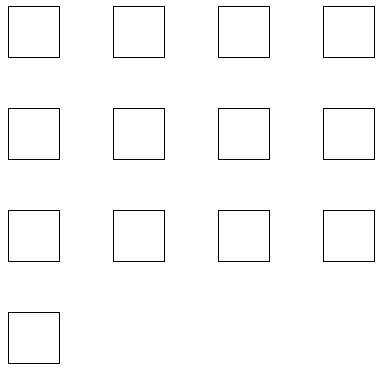
\includegraphics[scale=.4]{Bilder/AllocRes.png}
\captionof{figure}{Result Allocation of 13 Collapsables}
\end{figure}

The reason is that the \emph{CollapsableRule} shown next goes from 0 to limit (resulting in 4 spots) to make sure there are enough spots for all collapsables.

Afterwards the placement rule will use this limit to allocate the nodes in lines, starting at \emph{(0, 0)}.
\begin{lstlisting}[caption={Placing all Collapsables}]
export const CollaspableRule = ( node, allCollapsables, client, limit, minDist = 1000 ) => {
	if ( isCollapsable( node ) ) {
		const otherCollapsables = allCollapsables.filter( aNode => aNode.id !== node.id && !aNode.deleted );
		const existingCoords = getExistingCoordinatesFor( otherCollapsables );
		let newCoords = {};

		loop1:
		for ( let i = Math.floor( existingCoords.length / limit ); i <= limit + 1; i++ ) {
			for ( let j = existingCoords.length % limit; j <= limit; j++ ) {
				newCoords = { x: j * minDist, y: i * minDist };
				if ( !coordsExist( newCoords, existingCoords ) ) {
					node.position = newCoords;
					break loop1;
				}
			}
		} 
	}
}
\end{lstlisting}
This code does not include any comments or error handling to shorten it.

\newpage
\subsubsection{FlowerRule}
Afterwards the nodes around the collapsables are placed. 

If the parent has a level of \emph{0} it is a collapsable. The first position for a node is defined as the top-left (direction vector of \emph{(-1, -1)} from the parent). The delta angle between child nodes is calculated by dividing 360 by the number of children. Then it'll get the index of the current children in the list of childs the parent has and multiply the delta angle by this index. It then rotates the initial direction vector to get the one pointing at the position of the node. Multiplying it with the distance calculated in respect to the amount of other children leads to the position of the node.

Should the parent be a node with a level other than 0 the new position depends on the parent's direction vector. All children can be placed within an angle of +-90 degrees in the direction of the parent's direction vector. The delta angle is again calculated by the total amount of child nodes. Calculating the new position works as with children of level 1. However as these nodes can have multiple parents the newly calculated position has to be added to the one the node might already have and get normalized afterwards. \\

\begin{lstlisting}[caption={Allocating Nodes around Collapsables}]
for ( let collapsable of collapsables ) {
	const next = [].concat( collapsable.children );
	FlowerRule( next, client );
}

export const FlowerRule = ( next, client, distanceToOther = 350, minDist = 150 ) => {
	const nodeToCalculate = next.shift();
	if ( nodeToCalculate ) {
		for ( let parent of nodeToCalculate.parents ) {
			if ( parent.level === 0 ) {
				const initVec = { x: -1, y: -1 };
				let normalized = normalizeVector( initVec );
				let deltaAngle = 360 / parent.children.length;
				if ( parent.children.length % 2 === 0 ) {
					deltaAngle = deltaAngle * 3 / 5;
				}
				const deltaRad = toRad( deltaAngle );
				const index = parent.children.indexOf( nodeToCalculate );
				normalized = rotateVector( normalized, index * deltaRad );
				nodeToCalculate.dirVector = normalized;
				if ( !nodeToCalculate.position ) {
					nodeToCalculate.position = { x: 0, y: 0 };
				}
				const distance = calcDistance( nodeToCalculate );
				const newCoords = {
					x: parent.position.x + normalized.x * clamp( distance, minDist ),
					y: parent.position.y + normalized.y * clamp( distance, minDist ),
				};
				nodeToCalculate.position = addVertex( nodeToCalculate.position, newCoords );
			}
			else {
				const { dirVector } = parent;
				const zeroVec = rotateVector( dirVector, toRad( -90 ) );
				const deltaAngle = 180 / parent.children.length;
				const deltaRad = toRad( deltaAngle );
				const initVec = rotateVector( zeroVec, deltaRad / 2 );
				let normalized = normalizeVector( initVec );
				const index = parent.children.indexOf( nodeToCalculate );
				normalized = rotateVector( normalized, index * deltaRad );
				nodeToCalculate.dirVector = normalized;
				if ( !nodeToCalculate.position ) {
					nodeToCalculate.position = { x: 0, y: 0 };
				}
				const distance = calcDistance( nodeToCalculate );
				const newCoords = {
					x: parent.position.x + normalized.x * clamp( distance, minDist ),
					y: parent.position.y + normalized.y * clamp( distance, minDist ),
				};
				nodeToCalculate.position = addVertex( nodeToCalculate.position, newCoords );
				if ( !nodeToCalculate.dirVector ) {
					nodeToCalculate.dirVector = { x: 0, y: 0 };
				}
				nodeToCalculate.dirVector = addVertex( nodeToCalculate.dirVector, normalized );
			}
		}
		normalizeCoords( nodeToCalculate );

		for ( let childNode of nodeToCalculate?.children ) {
			if ( !next.includes( childNode ) ) {
				next.push( childNode );
			}
		}
		FlowerRule( next, client );
	}
};
\end{lstlisting}
This code does not include any comments or error handling to shorten it.

\subsubsection{NonCollapsableRule}
The last rule handles all nodes that are not connected to a collapsable in any way and thus have not received any coordinates yet and it works in a very similar manner.

It'll find the node with most connections and place it on the top left of the collapsable at the origin. There is no specific reason for this position, it was simply defined like that. The next step is to create the parent-child hierarchy for this network and then apply the flower rule to it.

